\documentclass[12pt]{article}%
\usepackage[T1]{fontenc}%
\usepackage[utf8]{inputenc}%
\usepackage{lmodern}%
\usepackage{textcomp}%
\usepackage{lastpage}%
\usepackage[backend=biber]{biblatex}%
\usepackage{fancyhdr}%
\usepackage{lastpage}%
\usepackage{ragged2e}%
\usepackage{pdfpages}%
\usepackage{hyperref}%
\usepackage{setspace}%
\usepackage{booktabs}%
\usepackage{float}%
\usepackage{threeparttable}%
\usepackage{amssymb}%
\usepackage{amsmath}%
\usepackage{adjustbox}%
\usepackage{longtable}%
\usepackage{breqn}%
\usepackage{tabularx}%
\usepackage{graphicx}%
\usepackage{placeins}%
\usepackage{geometry}%
\usepackage{fancyhdr}%
%
\geometry{top=1in, bottom=1in, left=1in, right=1in, headheight=14.5pt}%
\addbibresource{references.bib}%
\hypersetup{colorlinks=true, linkcolor=blue, urlcolor=blue}%
\fancypagestyle{frontmatter}{%
\renewcommand{\headrulewidth}{0pt}%
\renewcommand{\footrulewidth}{0pt}%
\fancyhead{%
}%
\fancyfoot{%
}%
\fancyhf{}%
\fancyhead[L]{DV410}%
\fancyhead[C]{\thepage}%
\fancyhead[R]{23802}%
}%
\fancypagestyle{mainmatter}{%
\renewcommand{\headrulewidth}{0pt}%
\renewcommand{\footrulewidth}{0pt}%
\fancyhead{%
}%
\fancyfoot{%
}%
\fancyhf{}%
\fancyhead[L]{DV410}%
\fancyhead[C]{Page \thepage\ of \pageref{LastPage}}%
\fancyhead[R]{23802}%
}%
\setstretch{1.5}%
\justifying%
\pagenumbering{roman}%
\pagestyle{fancy}%
\fancyhf{}%
\fancyhead[L]{DV410}%
\fancyhead[C]{Page \thepage\ of \pageref{LastPage}}%
\fancyhead[R]{23802}%
%TC:ignore%
\title{
        \begin{flushright}
        \large \textbf{Candidate Number: 23802}
        \end{flushright}
        \vspace*{30mm}
        \begin{center}
        \large MSc in Development Management 2023 \\
        \large (Applied Development Economics Specialism) \\
        \vspace*{5mm}
        Dissertation submitted in partial fulfilment of the requirements of the degree. \\
        \vspace*{35mm}
        \large \textbf{Building and Stumbling Blocks: An Empirical Analysis of the Heterogenous Effects of Trade Agreements Between North and South Countries} \\
        \vspace*{20mm}
        \end{center}
    }%
\date{}%
%TC:endignore%
%
\begin{document}%
\normalsize%

\includepdf[pages=-, offset=0 -1cm, frame]{DV410_Dissertation Cover Sheet_ Consent Form_Front Page_2023-24.pdf}%
\pagestyle{frontmatter}%
\maketitle%

\vfill
\begin{center}\textbf{Word Count: 9310}\end{center}
\newpage%
%TC:ignore%
\vspace*{\fill}%
\begin{center}%
\begin{minipage}{0.8\textwidth}%
\begin{center}%
\section*{Abstract}%
\end{center}%
\justify%
Extensions to the Gravity Model of Trade are used to empirically estimate across regions the heterogeneous partial effects of Trade Agreements (TAs) signed between 2000 and 2010 on trade volumes and value per unit of manufacturing products exported, as well as the effects on North{-}North, North{-}South and South{-}South bilateral trade relationships. We find that the average “total” partial effects of TAs in the period studied are similar to the estimates of the relevant literature, but there are heterogeneous effects of specific agreements within regions both on trade volume and value per unit. We also find heterogeneous effects of TAs on the different categories of bilateral trade relationships. We conclude that TAs can have positive and negative effects on both North{-}South and South{-}South trade, and we explore potential mechanisms driving this heterogeneity.%
\end{minipage}%
\end{center}%
\vspace*{\fill}%
\vspace*{\fill}%
\begin{flushleft}%
\textbf{Keywords:} “Trade Agreements”; “South-South”; “North-South”; “International Trade”; “Exports”; “Export Product Unit Value”; “Gravity Model”.%
\end{flushleft}%
%TC:endignore%
\newpage%
%TC:ignore%
\newpage%
\begin{center}%
\section*{Acknowledgements}%
This work is dedicated to Lupe, Armando, Lupita and Pepe. Thank you for everything.%
\end{center}%
The Author is grateful for the financial support of the British Foreign, Commonwealth and Development Office Chevening Scholarship (2023/2024), and for the encouragement and patience of the Academic Staff at LSE Department of International Development.%
%TC:endignore%
\newpage%
\tableofcontents%
\newpage%
%TC:ignore%
\section*{Abbreviations}%
\label{sec:Abbreviations}%
\begin{tabbing}%
\hspace{3cm} \= \kill%
\textbf{CMs} \> Common Markets \\%
\textbf{COMTRADE} \> UN Commodity Trade Statistics Database \\%
\textbf{CU} \> Customs Union \\%
\textbf{DESTA} \> The Design of International Trade Agreements Database \\%
\textbf{EPUV} \> Export Product Unit Value \\%
\textbf{EUs} \> Economic Unions \\%
\textbf{FTA} \> Free Trade Agreements \\%
\textbf{HS} \> Harmonysed System \\%
\textbf{INDSTAT } \> UNIDO Industrial Statistics database \\%
\textbf{NRPTAs} \> Non-reciprocal Preferential Trade Agreements \\%
\textbf{PTAs} \> Preferential Trade Agreements \\%
\textbf{TAs} \> Trade Agreements \\%
\textbf{TradeProd} \> The Trade and Production Database \\%
\end{tabbing}

%
%TC:endignore%
\newpage%
%TC:ignore%
\listoffigures%
%TC:endignore%
\newpage%
%TC:ignore%
\listoftables%
%TC:endignore%
\newpage%
\pagenumbering{arabic}%
\pagestyle{mainmatter}%
\section{Introduction}%
\label{sec:Introduction}%
The proliferation of Trade Agreements (TAs) since the early 1990s has
been well documented in the international trade academic literature
(\cite{dahi_preferential_2013} Dahi \& Demir, 2013; \cite{mayda_south-south_2007} Mayda \& Steinberg, 2007). This trend has slowed
down since the 1990s but is has not stopped. Figure 1 shows the historical
evolution of TAs, showing the dramatic increase in the 1990s.%


\begin{figure}[h!]%
\centering%
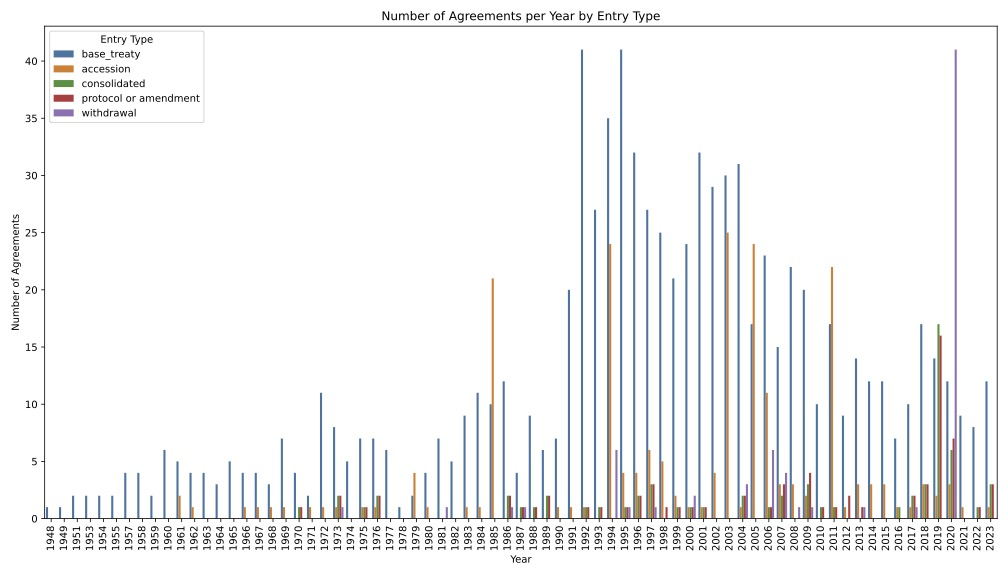
\includegraphics[width=0.8\textwidth]{figures/all_entries_agreements_per_year.jpg}%
\caption{Trade Agreements Per Year}%
\end{figure}

%
\FloatBarrier%
\textit{Source: Visualisation made by author. Data by The Design of International Trade Agreements Database (DESTA).}%
\FloatBarrier%
Moreover, the vast majority of TAs have been signed between developing countries, what is referred to as “South{-}South” trade cooperation, covering an increasingly important share of global trade across industries. Figure 2 shows the historical evolution of South{-}South TAs, Figure 3 shows the historical evolution of North{-}South TAs, and Figure 4 shows the historical evolution of North{-}North TAs, showcasing the significant difference in the number of agreements and countries belonging to each group.%


\begin{figure}[h!]%
\centering%
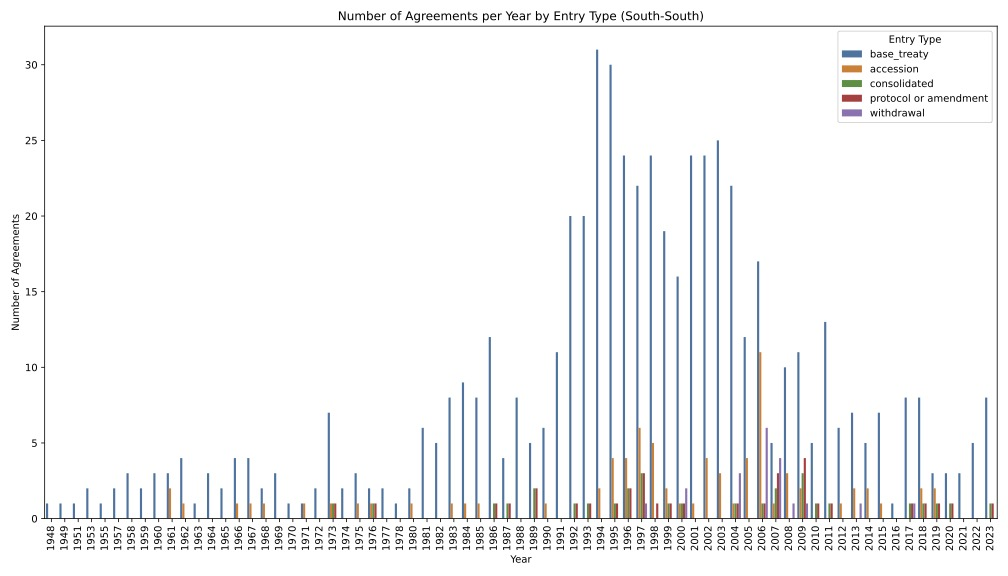
\includegraphics[width=0.8\textwidth]{figures/agreements_per_year_South-South.jpg}%
\caption{Trade Agreements Per Year (South{-}South).}%
\end{figure}

%
\FloatBarrier%
\textit{Source: Visualisation made by author. Data by The Design of International Trade Agreements Database (DESTA).}%
\FloatBarrier%


\begin{figure}[h!]%
\centering%
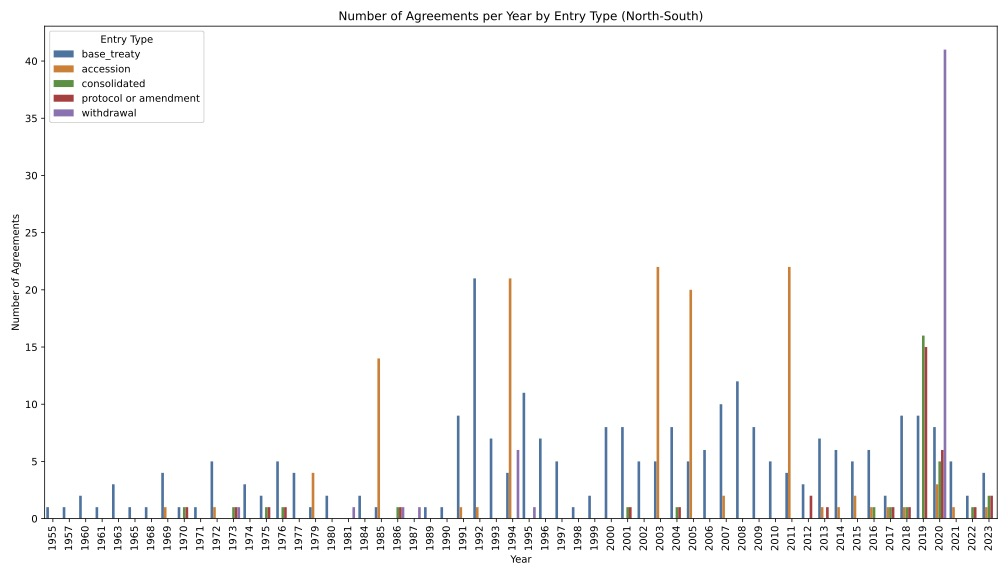
\includegraphics[width=0.8\textwidth]{figures/agreements_per_year_North-South.jpg}%
\caption{Trade Agreements Per Year (North{-}South).}%
\end{figure}

%
\FloatBarrier%
\textit{Source: Visualisation made by author. Data by The Design of International Trade Agreements Database (DESTA).}%
\FloatBarrier%


\begin{figure}[h!]%
\centering%
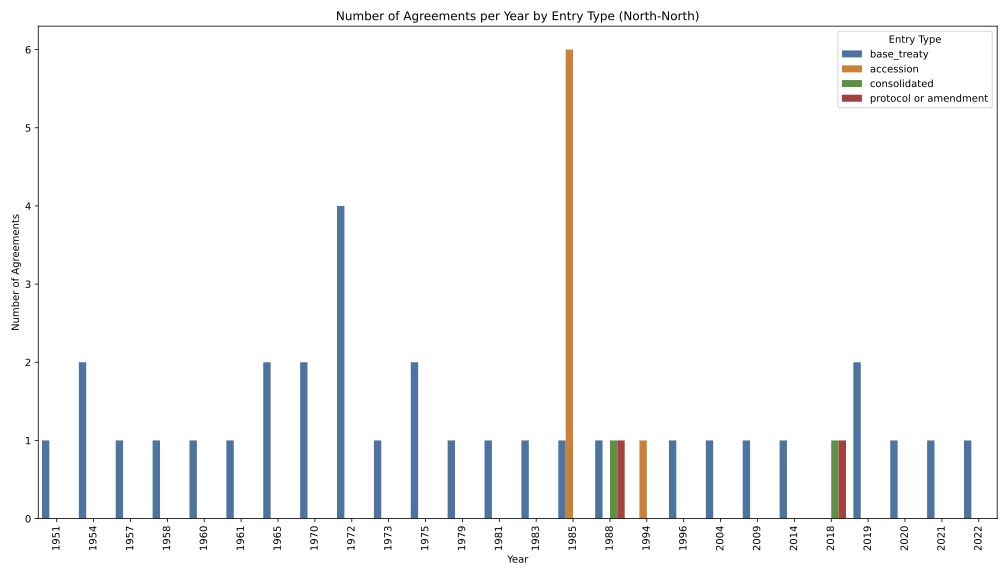
\includegraphics[width=0.8\textwidth]{figures/agreements_per_year_North-North.jpg}%
\caption{Trade Agreements Per Year (North{-}North).}%
\end{figure}

%
\FloatBarrier%
\textit{Source: Visualisation made by author. Data by The Design of International Trade Agreements Database (DESTA).}%
\FloatBarrier%
Despite their apparent importance for the governments of developing
countries, a common view in the academic literature is that South-South
TAs are not as effective as North-South TAs, or even that they do not
achieve significant effects, making them largely symbolic (\cite{gamso_leveling-up_2022} Gamso \&
Postnikov, 2022). North-South agreements, signed between developed and
developing countries, are presented as a superior alternative, more
effectively leading to increased trade for its members, and quality
upgrading through learning-by-exporting dynamics and better access to
intermediate goods for developing countries. At the same time, other
strands of the international trade literature present South-South TAs as
a more effective platform for developing countries to grow, at least to
a level where they can take advantage of North-South cooperation without
being undermined by more influential powers. This debate is often
presented as a dichotomy, where South-South TAs are either building or
stumbling blocks for developing countries. Solving it will go a long
way in better informing developing countries into which agreements they
should enter, with what types of partners, and how should the agreement
be designed.

In this paper, we venture to analyse this dichotomy empirically through
the use of a gravity model of trade, and subsequent extensions, in order
to get estimates for the effects of specific TAs, as well as estimates
on the effects of TAs on South-South, North-South and North-North
bilateral trade relationships, relative to non-TA-members. We also
explore the use of the export product unit value (EPUV) as an
alternative to trade volume, in order to capture the effects of TAs on
the value per unit exported of manufacturing goods. As such, we aim to answer
two specific research questions: do South-South TAs act as building
blocks or stumbling blocks to developing countries? Are they preferable
to North-South agreements?

This research is related to literature from traditional trade theory on
comparative advantage, to new trade theory and classical development
theory on the potential dynamic and scale effects of TAs, and to more
recent literature on the relevance of the structure of the product space
exported and the extensive margin of trade.

The paper proceeds in section 2 with a review of the relevant
theoretical and empirical literature on the effects of TAs on
North-South and South-South trade and potential development
implications. Section 3 introduces our empirical methodology and data.
Section 4 presents and describes our main findings, and Section 5
analyses and discusses their potential implications and how they fit
within the relevant literature. Finally, Section 6 concludes.

%
\section{Literature Review}%
\label{sec:LiteratureReview}%
This section reviews the literature on the theoretical and empirical potential effects of TAs on exports and welfare and situates the analysis in the relevant field of research.%
\subsection{Theoretical Framework}%
\label{subsec:TheoreticalFramework}%
The relevant theoretical framework in the literature is often described as a dichotomy, where TAs are either stumbling or building blocks in the development path of developing countries.%
\subsubsection{Comparative Advantage and Trade Creation and Diversion}%
\label{ssubsec:ComparativeAdvantageandTradeCreationandDiversion}%

%
Traditional trade theory emphasizes trade creation (allowing cheaper
products from TA members to substitute for more expensive domestic
products) and trade diversion (substituting products from non-TA members
that were cheaper before the TA with products from TA members that are
cheaper now due to the TA reducing tariffs) (\cite{schiff_regional_2003} Schiff, Winters and Schiff,
2003) and argues that the impact of TAs depends on the comparative
advantage of member countries. In particular, it argues that TAs magnify
the impacts of a country's comparative advantage, relative to the world
and to other member countries signatories of a common TA. If member
countries of a TA have a comparative advantage on a factor endowment
relative to the world, but one country also has a comparative advantage
on the same factor endowment relative to the other member countries, the
country with the ``extreme'' advantage will be more vulnerable to trade
diversion effects, while countries with ``intermediate'' advantages will
gain from trade creation effects, predicting divergence of trade
outcomes, and winners and losers among member countries. (\cite{venables_winners_2003} Venables,
2003). This emphasis on the trade creation and trade diversion effects
among member countries with significant differences in the comparative
advantage of their factor endowments relative to the world and to each
other, suggests that, when the country with the ``extreme'' comparative
advantage is a high-income country, relative to a lower-income country
with an ``intermediate'' comparative advantage, the lower-income country
should seek a TA with the other high-income country as it will gain
more. On the contrary, if both members are lower-income countries, the
country with the ``extreme'' comparative advantage, should not seek a TA
with the other low-income member country as it will be vulnerable.
(\cite{sanguinetti_impact_2010} Sanguinetti, Siedschlag and Martincus, 2010). This logic can be easily
extended to the North-South and South-South types of TAs, as ``North''
countries will reasonably have an ``extreme'' comparative advantage in
skill-intensive goods relative to ``South'' countries, while ``South''
countries will reasonably have an ``extreme'' comparative advantage in
labour-intensive goods relative to ``North'' countries. Furthermore, it
is also argued in the literature that benefiting from economies of scale
through South-South economic integration is more difficult because
member countries do not have complementary production and trade
structures, nor high interpenetration of each other's markets on
intra-industry trade. (\cite{schiff_regional_2003} Schiff, Winters and Schiff, 2003). Also, South
countries can benefit from greater technological diffusion from
North-South TAs as the ``North'' countries have higher industrial
development as well as investment in research (\cite{schiff_north-south_2008} Schiff and Wang, 2008).
Finally, as the trend in manufacturing has been in favour of vertical
specialization or value chain fragmentation (\cite{krugman_growing_1995} Krugman, 1995), North-South
TAs are preferable as developing countries strive to capture a greater
portion of the value added. Based on these arguments, developing
countries should therefore be better off entering into North-South
rather than South-South agreements.%
\subsubsection{Economies of Scale, Input{-}Output linkages and Products Exported}%
\label{ssubsec:EconomiesofScale,Input{-}OutputlinkagesandProductsExported}%

%
In contrast, classical development theory and new trade literature go
beyond the static welfare gains from trade creation and diversion
effects when analysing the effect of TAs. Developing countries can use
TAs to overcome limitations of their domestic market size in the
industrialisation process (\cite{dahi_preferential_2013} Dahi and Demir, 2013). Such potential
increases in the effective market size could help industries in
developing countries achieve economies of scale and increase the skill
content of production and exports, which in turn could improve the
market penetration of exports of developing countries in developed
markets in industrial products (\cite{fugazza_can_2006} Fugazza and Robert-Nicoud, 2006). Also,
due to similarities in production patterns and resource base among
developing countries, incentivising trade by lowering barriers could
facilitate appropriate technology transfer, according to the needs of
developing countries (\cite{unido_industrial_2006} UNIDO, 2006). Of particular relevance for
developing countries, it is argued that the products that countries
export matter for long-term economic performance. If a country exports
products from industries that are more technology-intensive, these are
likely to create input-output linkages and spillover effects in human
and physical capital accumulation and innovation (\cite{hausmann_what_2007} Hausmann, Hwang and
Rodrik, 2007). Furthermore, by allowing for factor accumulation, TAs can
reduce intra-block trade barriers and increase competition and access to
cheaper intermediate goods, triggering changes in industrial production
in member countries. As such, TAs among ``South'' countries can reduce
intra-South barriers and lead to industrialization of the region (\cite{puga_trading_1998} Puga
and Venables, 1998). In this context, what matters are not static gains
from TAs, but dynamic gains in industrial development. If South-South
TAs truly promote industrial development of member countries, they might
be desirable even if there are short-term losses due to trade diversion
(\cite{dahi_preferential_2013} Dahi and Demir, 2013). Other arguments in the development literature
emphasize the asymmetries in bargaining power between ``North'' and
``South'' countries, which could lead to worse outcomes for developing
countries if their policy space gets restricted (\cite{thrasher_21st_2008} Thrasher and Gallagher,
2008). To the extent that these arguments hold true, developing
countries could be better off entering into South-South rather than
North-South agreements, or at least should pursue both kinds of
agreements.

%
\subsection{Relevance of the Structure of Product Space}%
\label{subsec:RelevanceoftheStructureofProductSpace}%

%
As a compliment to trade theory, new trade theory and classical
development theory, there is a recent strand of the academic literature
that emphasises the importance of the structure of the product space
exported by each country in the structural transformation process.
Beyond factor endowments of physical, human and institutional capital,
and their subsequent evolution through accumulation processes, as the
basis for the comparative advantage of countries, this literature
proposes and finds evidence of patterns of path dependence depending on
the current capabilities of countries, and the relatedness of current
capabilities to the capabilities required to produce new products in the
future (\cite{hausmann_structure_2007} Hausmann and Klinger, 2007). As it is observed that human
capital for one product is imperfectly substitutable for other products,
and the degree of substitutability determines the relatedness of
products, the implication is that, as countries experience a strong
tendency to move into related products that require the capabilities
that a country already has or that are similar, the opportunities for
future transformation are dictated by the current product space and its
proximity to related products. Moreover, it also implies that there is a
positive exponential relationship between the returns to the
accumulation of new capabilities and the capabilities present in a
country. (\cite{hausmann_country_2010} Hausmann and Hidalgo, 2010). The more diverse the product
structure of a country, the higher the returns to accumulate new
capabilities. Inversely, we can find a ``trap of economic stasis'', in
which countries with few capabilities have little incentives to
accumulate new capabilities as they will have negligible or no returns,
predicting a world of divergence in industrial development. Furthermore,
this literature suggests that countries converge to the level of income
determined by their productive structures and how complex they are
(\cite{hidalgo_building_2009} Hidalgo and Hausmann, 2009). An underlying assumption of this
literature is that what a country exports matter and signals valuable
information about a country's comparative advantage and productive
structure, not only on its current industries and capabilities, but also
on a component of the evolution of its comparative advantage based on
the relatedness to other industries and capabilities (\cite{hausmann_implied_2014} Hausmann \emph{et
al.}, 2014). The implications of this literature to the effects of TAs
appears to be relevant to the extent that TAs can help countries acquire new
capabilities and diversify their structure of product space. Logically,
although North-South trade has the largest potential to allow South
countries to acquire new capabilities, we expect that the highest
returns should be made by acquiring capabilities in industries and
products related to the current capabilities of countries, which in the
context of our research should occur between countries with related
productive structures. As such, South-South trade could function as a
building block for developing countries to acquire new capabilities and
diversify the structure of their product space, before they can take
advantage of acquiring new capabilities through North-South trade.%
\subsection{Empirical Evidence}%
\label{subsec:EmpiricalEvidence}%

%
The preference of a type of partner in a TAs then becomes an empirical
question. Do South-South TAs promote trade and industrial development
among their members? The empirical literature overall reports positive
effects of TAs on the trade of member countries, but with considerable
heterogeneity on the estimation coefficients. For example, a
meta-analysis of research papers on the effects of TAs on member trade,
encompassing 85 papers and 1827 estimates, finds an average of 0.59 (an
80\% increase in trade), with a median of 0.38 (a 46\% increase in
trade), a wide range of coefficient estimates (-9.01 to 15.41), and only
312 out of 1827 estimates reported as negative (\cite{cipollina_reciprocal_2010} Cipollina and Salvatici,
2010). Furthermore, a survey of the empirical research on the effect of
economic integration agreements on international trade flows, as well as
using the most modern econometric techniques to address biases, found an
increase of 50\% on international trade, but with significant variation
in the effects of specific agreements (\cite{kohl_we_2014} Kohl, 2014). However, much of the
empirical research is focused on the effects of TAs on or including the
most advanced economies. Empirical research focused exclusively on the
effects of South-South TAs or comparing them to the effects of
North-North or North-South TAs, is much less prevalent in the
literature. Although, several research papers do control for the type of
agreement (North-South or South-South) and have found positive and
significant effects of South-South TAs (\cite{medvedev_preferential_2006} Medvedev, 2006; \cite{mayda_south-south_2007} Mayda and
Steinberg, 2007; \cite{dahi_preferential_2013} Dahi and Demir, 2013; \cite{deme_trade-creation_2017} Deme and Ndrianasy, 2017), these
articles tend to be limited in their scope, sample size or only focus on
trade volumes. Using firm-level data, empirical literature studying
trade outcomes using unit values of exports reports evidence of the
value per unit increasing as the income level of the importing nation
increases (\cite{hallak_product_2006} Hallak, 2006; \cite{bastos_quality_2010} Bastos and Silva, 2010). Relevant to our
analysis, one article finds evidence that the same firms export their
products at a higher value per unit the higher the income level of the
importing nation (\cite{manova_export_2012} Manova and Zhang, 2012). Beyond providing evidence
that the direction of trade has immediate repercussions, this could also
provide evidence in favour of North-South TAs, as they can generate more
revenue and promote quality upgrading (\cite{dahi_south-south_2017} Dahi and Demir, 2017). At the
same time, other strands of the empirical research literature emphasise
the importance of similarities in trade structure and preferences and
provide evidence that countries of similar levels of income, technology
and endowments have higher levels of trade, and importantly, more
potential for convergence and spillovers (\cite{hallak_product-quality_2010} Hallak, 2010). Important for
our discussion of the structure of product space, empirical research
finds that trade between similarly endowed countries have more
diversified exports between them, relative to trade with countries with
different endowments (\cite{regolo_export_2013} Regolo, 2013), and that countries with neighbours
with shared or similar comparative advantages will experience an
increase in the export of similar products to the neighbouring country
(\cite{bahar_neighbors_2014} Bahar, Hausmann and Hidalgo, 2014). If similarity between countries is
highly relevant for knowledge transfer, South-South TAs can potentially
be more beneficial for developing countries.

%
\section{Methodology}%
\label{sec:Methodology}%
\subsection{Empirical Strategy}%
\label{subsec:EmpiricalStrategy}%
\subsubsection{The Gravity Model of Trade}%
\label{ssubsec:TheGravityModelofTrade}%

%
Often referred as the ``workhorse'' of international trade, the gravity
model is prominent in the empirical literature of applied international
trade analysis. Among the arguments that could support the use of the
gravity model, there are four that are particularly relevant for our
purposes. First, the gravity model of trade is intuitive to understand.
Following the metaphor of Newton's Law of Universal Gravitation, it
predicts that international trade between two countries is directly
proportional to the product of their economic size, and inversely
proportional to trade frictions between them. In simpler words, the
bigger (smaller) the economies of two countries, and the easier (harder)
it is for them to trade with each other, the more (less) we expect them
to trade. Second, it is referred to as a structural model with solid
theoretical foundations, which makes it appropriate for counterfactual
analysis, such as measuring the effects of trade policies as we aim to
do with the effects of North-South versus South-South agreements. Third,
the model has a flexible structure, which will allow us to construct a
specification tailored to our research. Finally, fourth, it holds
consistent and remarkable predictive power, both with aggregate and
sectoral data (\cite{yotov_advanced_2016} Yotov et al. 2016).

Through the decades, the gravity equation has been regularly upgraded in
the theoretical and empirical literature. Of relevance, the simple
intuition of the gravity model was theoretically extended by Anderson to
note that, after controlling for size, the increase or decrease is
\emph{relative} to the average barriers of the two countries with all
their partners, which are referred as ``multilateral resistance''
(\cite{anderson_theoretical_1979} Anderson 1979). The more trade barriers or resistance to trade exists
with other countries relative to a given partner, the more a country is
pushed to trade with said partner. Anderson also introduced the
assumptions of product differentiation by place of origin, and Constant
Elasticity of Substitution (CES) expenditures, or the Armington-CES
assumption (\cite{yotov_advanced_2016} Yotov et al. 2016; \cite{chatzilazarou_trade_2023} Chatzilazarou and Dadakas 2023), which
led us to today's generalized form of the gravity equation, as developed
and popularised by Anderson and van Wincoop (\cite{anderson_gravity_2003} Anderson and van Wincoop
2003).

Equally important, several empirical developments have strengthened the
gravity model and inform our choice of methodology: Exporter-time and
importer-time fixed effects are used to account for the multilateral
resistance terms in a gravity estimation with panel data (\cite{olivero_dynamic_2012} Olivero and
Yotov 2012). As the gravity model is often estimated with an OSL
estimator, zero-trade flows were dropped from the sample when trade was
transformed into a logarithmic form. Also, trade data is recognized to
suffer from heteroscedasticity (\cite{yotov_advanced_2016} Yotov et al. 2016). To solve for
zero-trade flows and heteroscedasticity, the Poisson Pseudo Maximum
Likelihood (PPML) estimator has been proposed to estimate the gravity
model, avoiding potential biases (\cite{silva_log_2006} Silva and Tenreyro 2006; \cite{santos_silva_further_2011} Santos Silva
and Tenreyro 2011). Country-pair fixed effects have been proposed to
account for the unobserved endogeneity of trade policy (\cite{baier_free_2007-1} Baier and
Bergstrand 2007). It is worth noting that the inclusion of
exporter-time and importer-time fixed effects will absorb all observable
and unobservable time-varying country-specific characteristics that
could affect the dependent variable, while the country-pair fixed
effects will absorb observable and unobservable bilateral time-invariant
characteristics that could affect trade costs between the country pair. The inclusion of
intra-trade flows as well as international trade flows is proposed to
correctly estimate the effects of non-discriminatory trade policy,
allowing for consumers to choose products from both international and
domestic sources (\cite{dai_trade-diversion_2014} Dai, Yotov, and Zylkin 2014; \cite{heid_estimating_2017} Heid, Larch, and Yotov
2017). Year-intervals instead of data pooled over consecutive years
should be used to allow for adjustment of trade flows to policies that
might not have immediate effects, as we expect TAs effects to behave (\cite{baier_free_2007-2} Baier and Bergstrand 2007; \cite{anderson_terms_2016-1} Anderson
and Yotov 2016). And finally, to account for the effects of
globalisation forces that may biased the estimates of trade policies, a
set of globalisation dummies are recommended to control for the effects
of globalisation in the gravity model (\cite{yotov_simple_2012} Yotov 2012; \cite{bergstrand_economic_2015} Bergstrand, Larch,
and Yotov 2015).%
\subsubsection{Benchmark Model}%
\label{ssubsec:BenchmarkModel}%

%
Based on the theoretical and empirical best-practices found in the
relevant literature, we employ the following gravity equation using a
PPML estimator and a balanced panel data approach with multiple
exporters, multiple importers and time as our benchmark model:

\begin{multline}
    X_{ij,t} = \exp\left(\eta_{i,t} + \psi_{j,t} + \gamma_{i,j} + \beta_{1} \, TA_{ij,t} \right. + \beta_{2} \, TA_{ij,t-5} + \left. \sum_{t} b_{t} \right) + \epsilon_{ij,t}
\end{multline}

Where \(X_{ij,t}\) denotes the value of exports from an origin country
\(i\) to a destination country \(j\); \(\eta_{i,t}\) and \(\psi_{j,t}\)
are, respectively, exporter-time and importer-time fixed-effects;
\(\gamma_{i,j}\) is a country-pair fixed-effect;
\({TA}_{ij,t}\) and \({TA}_{ij,t - 5}\) are our main variables of
interest, which, respectively indicate if \(i\) and \(j\) are members of
a TA at time \(t\) and, to account for potential ``phase-in'' effects
over time of the TA, at time \(t - 5\); \(\sum_{t}^{}b_{t}\) is a set of
dummies that equal 1 for international trade and 0 for domestic trade
observations at each time \(t\); and \(\epsilon_{ij,t}\) is an error
term.%
\subsubsection{TA Heterogeneity Model}%
\label{ssubsec:TAHeterogeneityModel}%

%
In contrast with our main interest of research, which are the potential
heterogenous effects of TAs on different members for different types of
agreements, this benchmark model, specifically
\(\beta = \beta_{1} + \beta_{2}\) , would provide the average ``total''
partial effect of TAs on trade, relative to non-TA-members, after accounting for lagged effects, but
it cannot provide the effects for a given agreement. As such, an
expansion can be implemented to capture heterogeneity in TA effects as
proposed by Baier \emph{et al}. (\cite{baier_widely_2019} Baier, Yotov, and Zylkin 2019):

\begin{multline}
    X_{ij,t} = \exp\left(\eta_{i,t} + \psi_{j,t} + \gamma_{i,j} + \sum_{A} \beta_{1,A} \, TA_{ij,t} \right. + \sum_{A} \beta_{2,A} \, TA_{ij,t-5} + \left. \sum_{t} b_{t} \right) + \epsilon_{ij,t}
\end{multline}

Equation (2) can be implemented to account for heterogeneous effects of
TAs at the level of the specific agreement, by allowing for distinct
average partial effects for each individual agreement, using superscript
\(A\) to index by agreement and also allowing for agreement-specific
lags: \(\beta_{A} = \beta_{1,A} + \beta_{2,A}\).%
\subsubsection{North{-}North, North{-}South and South{-}South TAs}%
\label{ssubsec:North{-}North,North{-}SouthandSouth{-}SouthTAs}%

%
In order to analyse the differentiated effects of North-North,
North-South and South-South TAs, we extend both models to get estimates
for each type of TA. Our benchmark model is extended as follows:

\begin{multline}
    X_{ij,t} = \exp\left(\eta_{i,t} + \psi_{j,t} + \gamma_{i,j} + \beta_{1NN} \, TA\_NN_{ij,t} + \beta_{2NN} \, TA\_NN_{ij,t-5} \right. \\
    + \beta_{1NS} \, TA\_NS_{ij,t} + \beta_{2NS} \, TA\_NS_{ij,t-5} + \beta_{1SS} \, TA\_SS_{ij,t} + \beta_{2SS} \, TA\_SS_{ij,t-5} \\
    + \left. \sum_{t} b_{t} \right) + \epsilon_{ij,t}
\end{multline}

Where \(X_{ij,t}\)\hspace{0pt} denotes the value of exports from country
\(i\) to country \(j\) at time \(t\); \(\eta_{i,t}\) and
\(\psi_{j,t}\ \)are exporter-time and importer-time fixed effects,
respectively; \(\gamma_{i,j}\) is a country-pair fixed effect;
\hspace{0pt}\(\beta_{1NN}\) and \(\beta_{2NN}\) are the coefficients for
the immediate and lagged effects of a North-North TA (\(TA\_ NN\));
\hspace{0pt}\hspace{0pt}\(\beta_{1NS}\) and \(\beta_{2NS}\) are the
coefficients for the immediate and lagged effects of a North-South TA
(\(TA\_ SN\)); \hspace{0pt}\hspace{0pt}\(\beta_{1SS}\) and
\(\beta_{2SS}\) are the coefficients for the immediate and lagged
effects of a South-South TA (\(TA\_ SS\)); \(\sum_{t}^{}b_{t}\) is a set
of time dummies accounting for international trade-specific effects at
each time \(t\); and \(\epsilon_{ij,t}\) is the error term.

Equation (2) also gets extended to capture the heterogeneous effects of
the different types of TAs as follows:

\begin{multline}
    X_{ij,t} = \exp\left(\eta_{i,t} + \psi_{j,t} + \gamma_{i,j} + \sum_{A}\left(\beta_{1,A,NN} \, TA\_NN_{ij,t} + \beta_{2,A,NN} \, TA\_NN_{ij,t-5}\right) \right. \\
    + \sum_{A}\left(\beta_{1,A,NS} \, TA\_NS_{ij,t} + \beta_{2,A,NS} \, TA\_NS_{ij,t-5}\right) + \sum_{A}\left(\beta_{1,A,SS} \, TA\_SS_{ij,t} + \beta_{2,A,SS} \, TA\_SS_{ij,t-5}\right) \\
    + \left. \sum_{t} b_{t} \right) + \epsilon_{ij,t}
\end{multline}

Where \(X_{ij,t}\)\hspace{0pt} denotes the value of exports from country
\(i\) to country \(j\) at time \(t\); \(\eta_{i,t}\) and
\(\psi_{j,t}\ \)are exporter-time and importer-time fixed effects,
respectively; \(\gamma_{i,j}\) is a country-pair fixed effect;
The summations \hspace{0pt}\(\sum_{}^{}A\) denote the sum over different
agreements \(A\) for: \(\beta_{1,A,NN}\) and \(\beta_{2,A,NN}\):
Coefficients for the immediate and lagged effects of North-North TAs
\hspace{0pt}(\(TA\_ NN\)); \(\beta_{1,A,NS}\) and \(\beta_{2,A,NS}\):
Coefficients for the immediate and lagged effects of North-South TAs
(\(TA\_ SN\)); \(\beta_{1,A,SS}\) and \(\beta_{2,A,SS}\): Coefficients
for the immediate and lagged effects of South-South TAs (\(TA\_ SS\));
\(\sum_{t}^{}b_{t}\) is a set of time dummies accounting for
trade-specific effects at each time \(t\); and \(\epsilon_{ij,t}\) is
the error term.

For both extended models we use the following variables:
\({TA\_ NN}_{ij,t}\) is a dummy variable that takes the value of 1 if
the trade pair \((i,j)\) is North-North and part of a TA at time \(t\),
and 0 otherwise; \({TA\_ NN}_{ij,t - 5}\) is a dummy variable that takes
the value of 1 if the trade pair \((i,j)\) is North-North and was part
of a TA at time \(t\)\emph{-5}, and 0 otherwise; \({TA\_ NS}_{ij,t}\) is
a dummy variable that takes the value of 1 if the trade pair \((i,j)\)
is North-South and part of a TA at time \(t\), and 0 otherwise;
\({TA\_ NS}_{ij,t - 5}\) is a dummy variable that takes the value of 1
if the trade pair \((i,j)\) is North-South and was part of a TA at time
\(t\)\emph{-5}, and 0 otherwise; \({TA\_ SS}_{ij,t}\) is a dummy
variable that takes the value of 1 if the trade pair \((i,j)\) is
South-South and part of a TA at time \(t\), and 0 otherwise;
\({TA\_ SS}_{ij,t - 5}\) is a dummy variable that takes the value of 1
if the trade pair \((i,j)\) is South-South and was part of a TA at time
\(t\)\emph{-5}, and 0 otherwise;

The extended models allow us to capture the differentiated effects of
TAs on bilateral exports depending on whether the pair country are two
``North'' countries (NN), a ``North'' and a ``South'' country (NS), or
two ``South'' countries (SS).

%
\subsection{Export Product Unit Value}%
\label{subsec:ExportProductUnitValue}%

%
Inspired by other strands of the international trade literature, we also
test our models using ``Unit Values'' of the products exported, by
dividing the total value exported by the total weight exported in
kilograms (\cite{latzer_average_2021} Latzer and Mayneris 2021; \cite{manova_export_2012} Manova and Zhang 2012; \cite{bastos_quality_2010} Bastos and
Silva 2010). Using the unit value as the dependent variable in our
estimations allow us to analyse if the value per unit exported is
affected by TAs. To be consistent in our effort to understand the
potentially heterogenous effects of TAs according to the different
category of the members in trade volume, but also in quality upgrading
and industrialization development of countries, we focus on
manufacturing products (\cite{chatzilazarou_trade_2023} Chatzilazarou and Dadakas 2023) with HS 2-digit
codes 84 (Nuclear reactors, boilers, machinery and mechanical
appliances; parts thereof ) and 85 (Electrical machinery and equipment
and parts thereof; sound recorders and reproducers, television image and
sound recorders and reproducers, and parts and accessories of such
articles) which are part of the ``Machinery and mechanical appliances;
electrical equipment; parts thereof; sound recorders and reproducers,
television image and sour sound recorders and reproducers, and parts and
accessories of such articles'' category from the World Customs
Organization. Our aim is to compare the effects of TAs on trade volumes
against the effects on the unit value of manufacturing products
exported.%
\subsection{Defining North and South}%
\label{subsec:DefiningNorthandSouth}%

%
Defining which countries belong to the ``North'' and ``South''
categories is a key step in order to properly analyse the impact of TAs
on different bilateral export relationships. However, it is important to
consider that any way in which we categorize countries can be criticised
for not taking into consideration the diverse and heterogenous
characteristics of individual countries within each group. Furthermore,
especially since our focus is to analyse South-South relationships, it
is possible to further disaggregate from the ``South'' group the
emerging economies which are becoming more relevant at the political and
economic world stage and are challenging the hegemony of traditional
developed economies. The level of disaggregation, as well as the level
of attention to heterogenous characteristics among and within groups,
depends on the research question at hand. For the purposes of this
paper, we will not consider such heterogeneity within groups, and just
focus on categorising countries as ``North'' and ``South'', but by no
means does this assumes that countries are homogenous within groups.
This is just a useful distinction to study heterogeneity across TA
effects.

One intuitive approach could be to categorize countries based on their
income level, but this approach would need to deal with a dynamic list
of groups, as countries change their category through time. Also,
high-income countries include non-industrialized small-nations which we
do not expect to generate significant effects on the industrial
development as well as technology- and skills-upgrading of trade-partner
countries. For such reasons, we have decided to use the same
categorization of countries as Dahi \& Demir (\cite{dahi_south-south_2017} Dahi and Demir 2017) which
takes into consideration characteristics such as incomes, production and
trade structures, factor endowments, and human and institutional
development to construct a list of ``North'' and ``South'' countries,
and also keeps the groups consistent over time. This results in 23
countries categorized as ``North'', and the rest as ``South''. A
detailed list of the countries and their categories can be found in the
Appendix I.%
\subsection{Data}%
\label{subsec:Data}%

%
To construct our dataset we have combined TA data from the ``Design of
International Trade Agreements'' (DESTA) (\cite{dur_andreas_leonardo_baccini_and_manfred_elsig_design_2014} Dür, Andreas, Leonardo Baccini
and Manfred Elsig 2014) and from the CEPII ``Trade and Production
Database'' (TradeProd) (\cite{thierry_mayer_gianluca_santoni_vincent_vicard_cepii_2023} Thierry Mayer, Gianluca Santoni, Vincent Vicard
2023). The DESTA database aims to aggregate all agreements that have the
potential to liberalise trade, including all agreements notified to the
World Trade Organisation (WTO) and other agreements from a wide range of
sources, covering 880 agreements for 204 countries since 1948 to 2023 in
the last updated version.

Our sample consists of TAs signed between the years 2000 to 2010 and the
country members to these TAs, totalling 154 agreements and 143 member
countries. For ease of estimation, and to get a sense of geographical
differences, we estimate our models by TA region for five main regions:
Africa, Americas, Asia, Europe and Intercontinental (We exclude Oceania
{[}11 countries and 1 agreement{]} for lack of sufficient trade data for
our estimations). Each region has the following samples of agreements
and countries: Intercontinental (114 countries and 64 agreements),
Europe (42 countries and 41 agreements), Asia (35 countries and 33
agreements), Americas (15 countries and 13 agreements) and Africa (10
countries and 2 agreements). A detailed list of the TAs in our sample and their 
member countries can be found in the Appendix II.

For all countries in our sample, we get international trade and domestic
trade flows from the TradeProd database, which has been created
specifically for estimating gravity models and combines trade data from
the UN Commodity Trade Statistics Database (COMTRADE) and production
data from UNIDO Industrial Statistics database (INDSTAT). We also
download export data directly from COMTRADE for all countries in our
sample to construct our export product unit value measurements. For
estimations on trade flows, we use international trade flow data as
reported by importer. In order to measure the appropriate lags for the
effects of each agreement, our period of interest for international flow
data is between 1995 to 2015, and since we are estimating in 5-year
intervals, we get trade flow data for the years 1995, 2000, 2005, 2010
and 2015. Finally, as mentioned before, export product unit values are
constructed using the total value exported per product per year divided
by the net weight exported of said product for said year at the HS
2-digit code level for the 84 and 85 codes for manufacturing products.
As it is not possible to get data for product unit values for domestic
trade, the estimations using this measure as the dependent variable will
suffer from bias as the estimation does not include intra-trade effects.
However, the direction of bias is important as not including intra-trade
measures is expected to bias the effects of TAs downwards (\cite{yotov_advanced_2016} Yotov et al.
2016), so we use this estimates as illustrative conservative
measurements of the effects of TAs on the unit value of exported
products.

%
\section{Findings}%
\label{sec:Findings}%
This section presents and describes the results of estimating our gravity models.

%
\subsection{Benchmark Results}%
\label{subsec:BenchmarkResults}%
We begin by briefly discussing the results of our benchmark estimation
by region, contained in Table 1. We immediately see that the average total or
``cumulative'' effects of TAs on trade flows, relative to non-TA-members, after accounting for
phase-in effects (the sum of the current and lagged TA estimates), is
heterogenous across regions. Only Americas, Europe and Intercontinental
TAs have statistically significant results, with all coefficients being
positive and generally similar to the results we would expect according
to the literature. The smallest effect, that of Intercontinental TAs,
has a statistically significant coefficient at the 5\% of 0.203 with a
standard error of (0.106). We interpret this coefficient as
Intercontinental TAs having an average a partial effect of
(exp(0.203)-1)x100\%. = 22.5\% increase in trade flows. The largest
effect, that of Europe's TAs, has a statistically significant
coefficient at the 1\% of 0.475 with a standard error of (0.025). We
interpret this coefficient as Europe's TAs having an average a partial
effect of (exp(0.475)-1)x100\%. = 60.8\% increase in trade flows. On the
other hand, Africa and Asia does not have statistically significant
results, with Asia's coefficient taking a negative value. Interestingly,
Africa's TA coefficient is highly significant and positive, and TA Lag
is not significant and negative, while Asia's TA coefficient is not
significant and positive, and TA Lag is highly significant and negative.
%
\begin{table}[htbp]
    \centering
    \caption{Benchmark Model Regional Results}
    \label{tab:benchmark_region_analysis} % This allows you to reference the table in the text with \ref{tab:pta_analysis}
    \begin{adjustbox}{max width=\textwidth}
    \begin{tabular}{l@{\extracolsep{1pt}}ccccc}
    \hline
    & \multicolumn{1}{c}{(1)} & \multicolumn{1}{c}{(2)} & \multicolumn{1}{c}{(3)} & \multicolumn{1}{c}{(4)} & \multicolumn{1}{c}{(5)} \\
    \hline
    \textbf{Variables} &  &  &  &  &  \\
    \hline
     & PPML & PPML & PPML & PPML & PPML \\
     & Africa & Americas & Asia & Europe & Intercontinental \\
    \hline
    PTA & 0.578$^{\ast\ast\ast}$ & 0.287$^{\ast\ast\ast}$ & 0.064 & 0.237$^{\ast\ast\ast}$ & 0.015 \\
    & (0.154) & (0.071) & (0.083) & (0.019) & (0.093) \\

    PTA Lag & -0.278 & 0.146 & -0.167$^{\ast\ast\ast}$ & 0.238$^{\ast\ast\ast}$ & 0.188$^{\ast\ast\ast}$ \\
    & (0.300) & (0.149) & (0.056) & (0.022) & (0.043) \\

    PTA + PTA Lag & 0.301 & 0.433$^{\ast\ast\ast}$ & -0.103 & 0.475$^{\ast\ast\ast}$ & 0.203$^{\ast}$ \\
    & (0.295) & (0.140) & (0.094) & (0.025) & (0.106) \\
    \hline
    Exporter-Year FE & Yes & Yes & Yes & Yes & Yes \\
    Importer-Year FE & Yes & Yes & Yes & Yes & Yes \\
    Country-Pair FE & Yes & Yes & Yes & Yes & Yes \\
    R-Squared & 0.997 & 0.999 & 0.999 & 0.997 & 0.998 \\
    Observations & 5838 & 10997 & 25308 & 28168 & 73930 \\
    \hline
    \multicolumn{6}{l}{\footnotesize{Notes: Robust standard errors clustered at the country-pair in parentheses. Significance levels are indicated as follows: $^{\ast}$p$<$0.1; $^{\ast\ast}$p$<$0.05; $^{\ast\ast\ast}$p$<$0.01.}} \\
    \end{tabular}
    \end{adjustbox}
\end{table}    %
\FloatBarrier

%
\subsection{TA Heterogeneity Results}%
\label{subsec:TAHeterogeneityResults}%
The results of our model allowing for heterogenous effects of TAs is
shown in Tables 15 through Table 19 in Appendix III. Again, we can
observe significant heterogeneity across regions and TAs. Africa in
Table 15 has no statistically significant effect for any TA. Americas in
Table 16 has ten TAs with statistically significant and positive
coefficients, two with no statistically significant effect, and one TA
with a statistically significant and negative coefficient. Asia in Table
17 has eight TAs with statistically significant and positive
coefficients, nine with no statistically significant effect, and four
TAs with statistically significant and negative coefficients. Europe in
Table 18 has eighteen TAs with statistically significant and positive
coefficients, nine with no statistically significant effect, and one TA
with a statistically significant and negative coefficient. And finally,
Intercontinental in Table 19 has twenty-eight TAs with statistically
significant and positive coefficients, twenty with no statistically
significant effect, and six TAs with statistically significant and
negative coefficients. Across the regions, 64 out of 118 (54.24\%)
coefficients have significant and positive effects, 42 out of 118
(35.59\%) have no significant effects, and 12 out of 118 (10.17\%) have
significand and negative effects. A summary of the findings can be found
on Figure 5, with the significance of the coefficients on the Y axis (all
non-significant coefficients assigned a value of -1 for ease of
visualization, and significant coefficients assigned a value of 1, 2 or
3 according to their significance, with the highest significance being
3) magnitude of the coefficients on the X axis, showing negative and
positive coefficients.
%


\begin{figure}[h!]%
\centering%
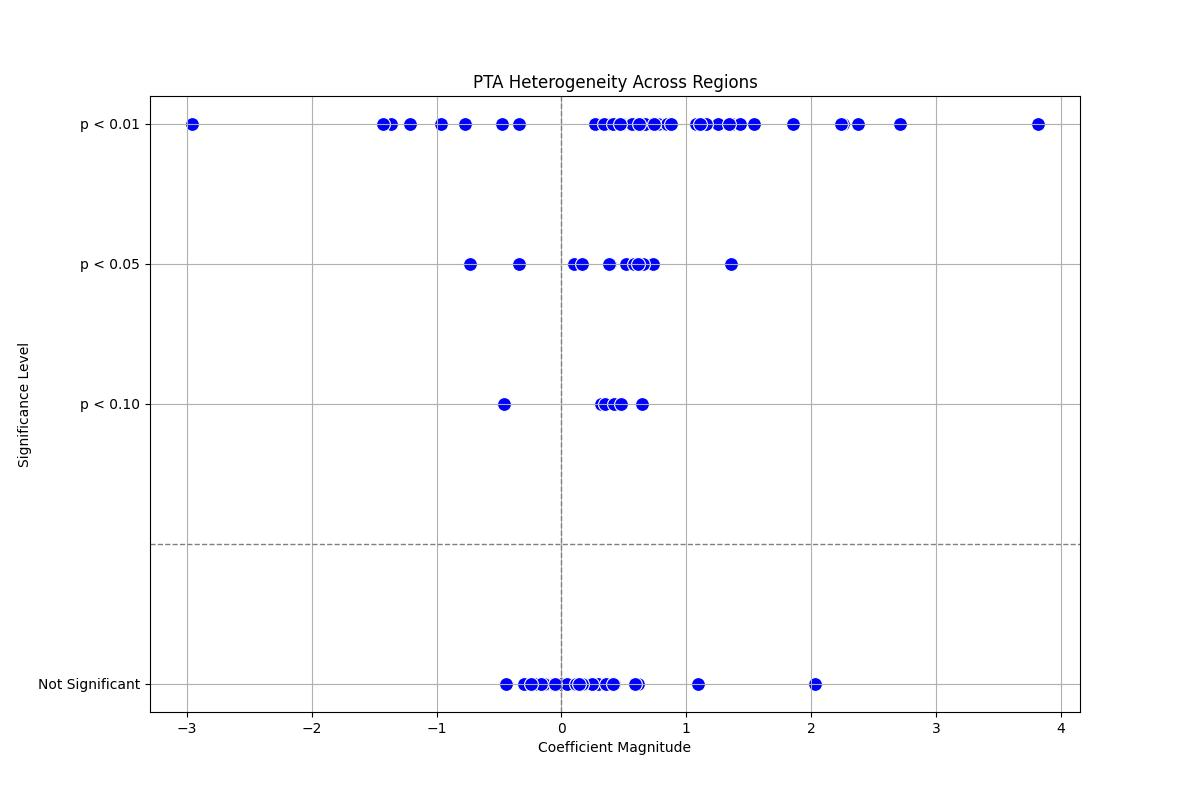
\includegraphics[width=0.8\textwidth]{figures/pta_het_vis.jpeg}%
\caption{TA Heterogeneity Across Regions}%
\end{figure}

%
\FloatBarrier

%
\subsection{North{-}North, North{-}South and South{-}South TAs}%
\label{subsec:North{-}North,North{-}SouthandSouth{-}SouthTAs}%
\subsubsection{North{-}South Benchmark Results}%
\label{ssubsec:North{-}SouthBenchmarkResults}%
We present the results of our extended models allowing us to capture the
differentiated effects of TAs on bilateral exports depending on whether
the country pair are two ``North'' countries (NN), a ``North'' and a
``South'' country (NS), or two ``South'' countries (SS).

The results of the extended benchmark estimation by region, contained in
Table 2 again show heterogenous results across regions. It is
interesting to note that by disaggregating the TA effects, in the case
of Americas and Europe, both of which had significant and positive
coefficients in the benchmark estimation, now again have significant and
positive coefficients for both NS TA + Lag and SS TA + Lag , but the
effects are larger in both cases for the SS TA + Lag coefficient. Asia
now has a slightly significant and negative coefficient for NS TA + Lag
while the coefficient for SS TA + Lag remains not significant.
Intercontinental have significant and positive effects of NS Lag and SS
Lag, but NS TA + Lag and SS TA + Lag are both not significant now.
Africa's coefficients remain not significant, and it is the only region
with only South-South TAs.
%
\begin{table}[htbp]
    \centering
    \caption{Regional Results by TA Type}
    \label{tab:pta_types}
    \begin{adjustbox}{max width=\textwidth}
    \begin{tabular}{lccccc}
    \hline
     & \multicolumn{1}{c}{Africa} & \multicolumn{1}{c}{Americas} & \multicolumn{1}{c}{Asia} & \multicolumn{1}{c}{Europe} & \multicolumn{1}{c}{Intercontinental} \\
    \hline
    \textbf{Variables} &  &  &  &  &  \\
    \hline
    NN TA &  &  &  & 0.207$^{\ast\ast\ast}$ & 0.013 \\
     &  &  &  & (0.021) & (0.072) \\
    NN TA Lag &  &  &  & 0.192$^{\ast\ast\ast}$ & 0.016 \\
     &  &  &  & (0.023) & (0.073) \\
    NN TA + NN TA Lag &  &  &  & 0.399$^{\ast\ast\ast}$ & 0.029 \\
     &  &  &  & (0.026) & (0.102) \\
    \hline
    NS TA &  & 0.199$^{\ast\ast\ast}$ & -0.089 & 0.374$^{\ast\ast\ast}$ & 0.013 \\
     &  & (0.069) & (0.089) & (0.041) & (0.144) \\
    NS TA Lag &  & 0.234 & -0.067 & 0.349$^{\ast\ast\ast}$ & 0.231$^{\ast\ast\ast}$ \\
     &  & (0.190) & (0.060) & (0.041) & (0.061) \\
    NS TA + NS TA Lag &  & 0.434$^{\ast\ast}$ & -0.156$^{\ast}$ & 0.723$^{\ast\ast\ast}$ & 0.244 \\
     &  & (0.200) & (0.090) & (0.046) & (0.156) \\
    \hline
    SS TA & 0.578$^{\ast\ast\ast}$ & 0.476$^{\ast\ast\ast}$ & 0.153 & 0.530$^{\ast\ast\ast}$ & 0.004 \\
     & (0.154) & (0.139) & (0.117) & (0.107) & (0.121) \\
    SS TA Lag & -0.278 & -0.023 & -0.208$^{\ast\ast\ast}$ & 0.575$^{\ast\ast\ast}$ & 0.204$^{\ast\ast\ast}$ \\
     & (0.300) & (0.133) & (0.063) & (0.119) & (0.073) \\
    SS TA + SS TA Lag & 0.301 & 0.453$^{\ast\ast\ast}$ & -0.055 & 1.105$^{\ast\ast\ast}$ & 0.208 \\
     & (0.295) & (0.112) & (0.130) & (0.092) & (0.128) \\
    \hline
    Exporter-Year FE & Yes & Yes & Yes & Yes & Yes \\
    Importer-Year FE & Yes & Yes & Yes & Yes & Yes \\
    Country-Pair FE & Yes & Yes & Yes & Yes & Yes \\
    R-Squared & 0.997 & 0.999 & 0.999 & 0.997 & 0.998 \\
    Observations & 5838 & 10997 & 25308 & 28168 & 73930 \\
    \hline
    \multicolumn{6}{l}{\footnotesize{Notes: Robust standard errors clustered at the country-pair level in parentheses.}} \\
    \multicolumn{6}{l}{\footnotesize{Significance levels are indicated as follows: $^{\ast}$p$<$0.1; $^{\ast\ast}$p$<$0.05; $^{\ast\ast\ast}$p$<$0.01.}} \\
    \end{tabular}
    \end{adjustbox}
\end{table}
%
\FloatBarrier

%
\subsubsection{North{-}South TA Heterogeneity Results}%
\label{ssubsec:North{-}SouthTAHeterogeneityResults}%
The results of our extended model allowing for heterogenous effects of
TAs is shown in Appendix IV in Tables 20 through Table 24. Africa in
table 20 only has effects for South-South TAs and again has no
statistically significant effect for any TA. Americas in Table 21 has
five TAs with North-South estimates, one of which has statistically
significant and negative effects for NS TA + Lag and statistically
significant and positive effects for SS TA + Lag. Of the remaining four,
none have estimates for SS TA + Lag, three are statistically significant
and positive, and one is not statistically significant. It has eight TAs
with South-South estimates, seven of which have statistically
significant and positive effects, while one does not have statistically
significant effects. Americas does not have any coefficients for
North-North. Asia in Table 22 has two TAs with North-South estimates,
one of which is statistically significant and positive, while the other
is not statistically significant. It has nineteen TAs with South-South
estimates, seven of which have statistically significant and positive
effects, four have statistically significant and negative coefficients,
and eight does not have statistically significant effects. Asia does not
have any coefficients for North-North. Europe in Table 23 has eight TA
North-South estimates, five of which are statistically significant and
positive, and the others are not statistically significant. One of the
five agreements with statistically significant and positive coefficients
for NS TA + Lag also has a statistically significant and positive
coefficient for SS TA + Lag. None of the other agreements with a NS
coefficient have statistically significant coefficients for SS. It has
nineteen South-South estimates, thirteen are statistically significant
and positive, one is statistically significant and negative, and five
are not significant. Finally, the region has one agreement with a
North-North estimate, which also has a North-South and a South-South
estimate and they are all statistically significant and positive.
Intercontinental in Table 24 has thirty TA North-South estimates, of
which twelve are statistically significant and positive, fifteen are not
statistically significant, and three are statistically significant and
negative for NS TA + Lag. None of these TAs also have coefficients for
SS TA + Lag of which five are statistically significant and positive,
three are not statistically significant, and one is statistically
significant and negative. It has twenty-one estimates for South-South,
of which fourteen are statistically significant and positive, five are
not statistically significant, and two are statistically significant and
negative. It has three agreements with North-North estimates, two
statistically significant and positive, and one are not statistically
significant. Across the regions and TAs, 23 out of 47 (48.94\%) NS
coefficients have significant and positive effects, 20 out of 47
(42.55\%) NS coefficients have no significant effects, and 4 out of 47 (8.51\%) NS
coefficients have significand and negative effects; 49 out of 84 (58.33\%) SS coefficients
have significant and positive effects, 27 out of 84 (32.14\%) SS coefficients have no
significant effects, and 8 out of 84 (9.52\%) SS coefficients have significand and
negative effects; and, 3 out of 4 (75\%) NN coefficients have
significant and positive effects, 1 out of 4 (25\%) NN coefficients have no significant
effects, and none have significand and negative effects. A summary of
the findings can be found on Figure 6 for North-South trade, Figure 7 for
North-North trade and Figure 8 for South-South trade, with the
significance of the coefficients on the Y axis (all non-significant
coefficients assigned a value of -1 for ease of visualization, and
significant coefficients assigned a value of 1, 2 or 3 according to
their significance, with the highest significance being 3) magnitude of
the coefficients on the X axis, showing negative and positive
coefficients.
%


\begin{figure}[h!]%
\centering%
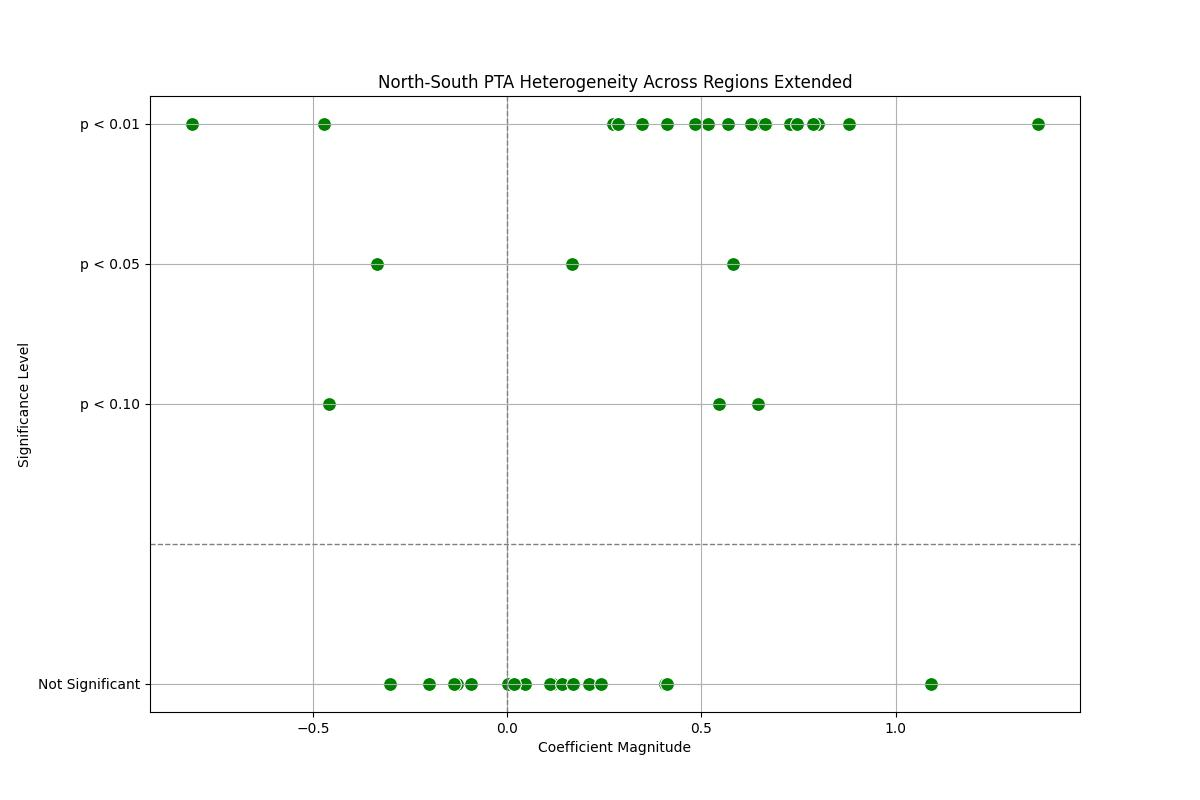
\includegraphics[width=0.8\textwidth]{figures/North-South_trade_relationships_visualization.jpeg}%
\caption{North{-}South TA Heterogeneity Across Regions Extended}%
\end{figure}

%


\begin{figure}[h!]%
\centering%
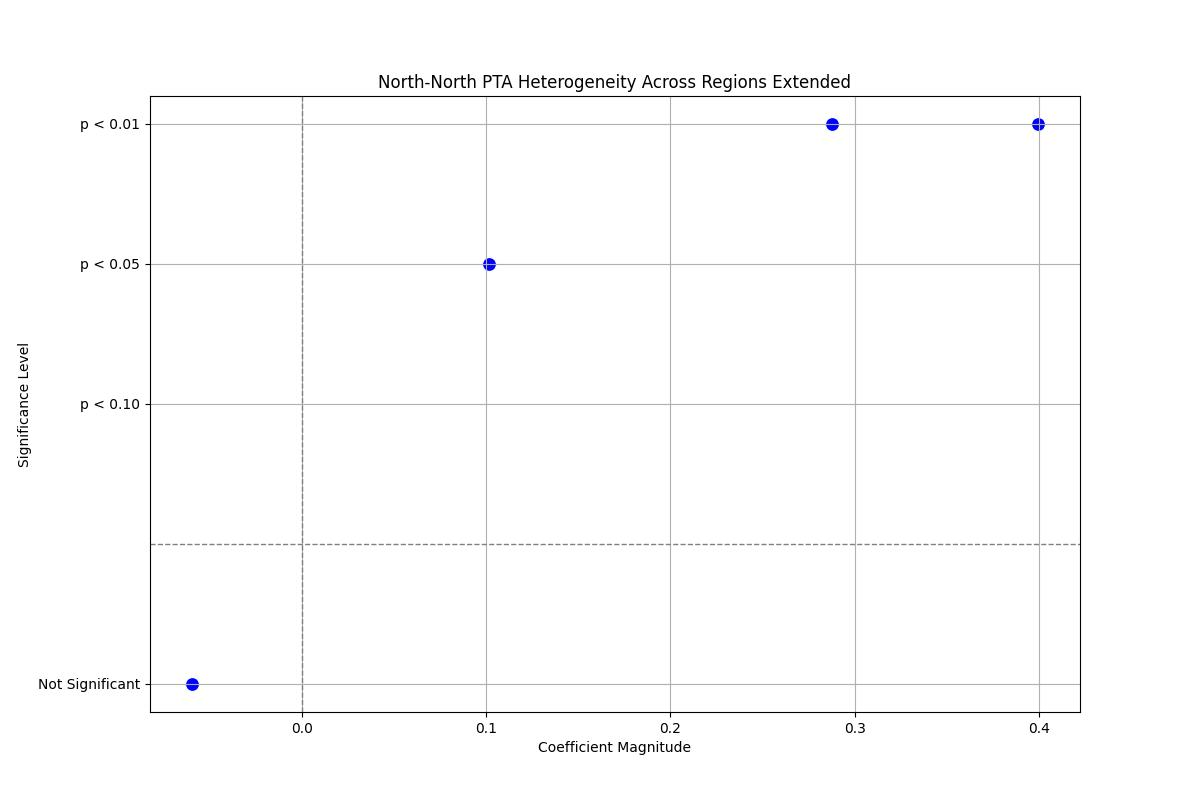
\includegraphics[width=0.8\textwidth]{figures/North-North_trade_relationships_visualization.jpeg}%
\caption{North{-}North TA Heterogeneity Across Regions Extended}%
\end{figure}

%


\begin{figure}[h!]%
\centering%
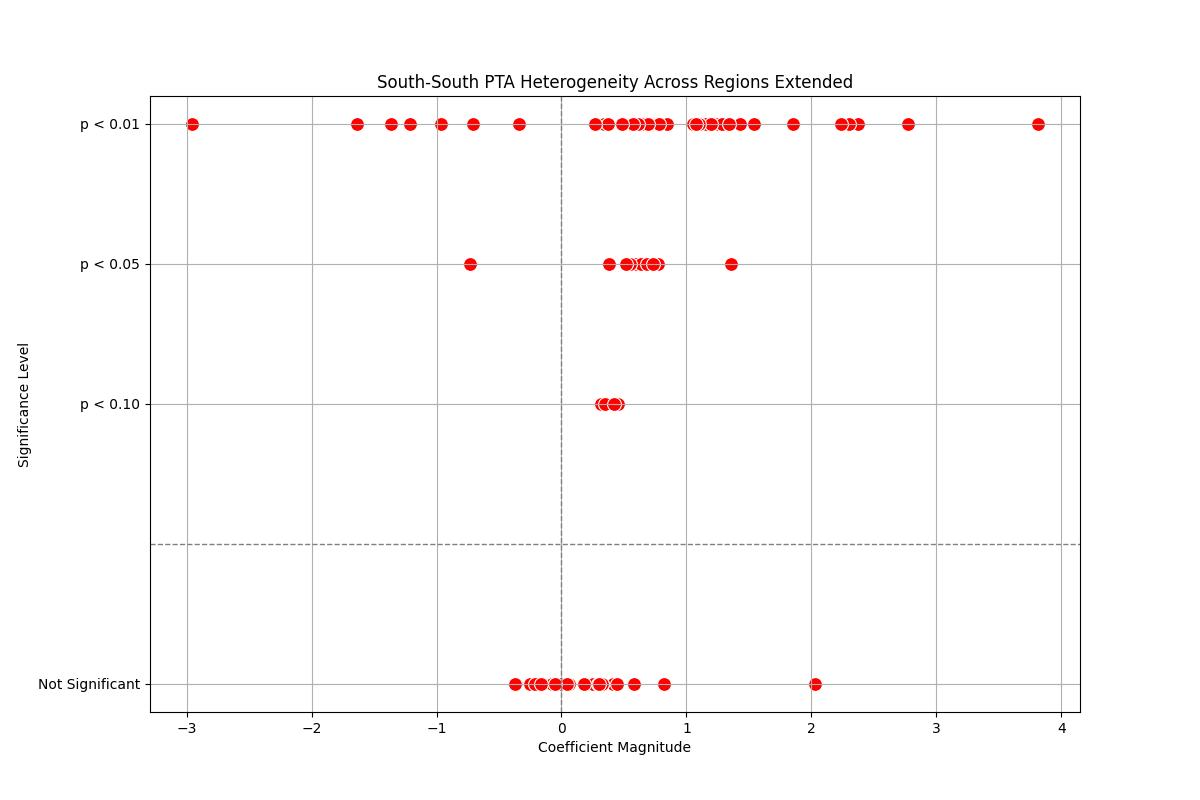
\includegraphics[width=0.8\textwidth]{figures/South-South_trade_relationships_visualization.jpeg}%
\caption{South{-}South TA Heterogeneity Across Regions Extended}%
\end{figure}

%
\FloatBarrier

%
\subsection{Export Product Unit Value Results}%
\label{subsec:ExportProductUnitValueResults}%
Finally, we present the results of running our estimations substituting
trade flows as our dependent variable for the unit values of products
exported, specifically under the HS 2-digit codes 84 and 85 for
manufacturing products, in order to analyse if the effect of TAs goes
beyond trade volumes. For ease of comparison, we ran each estimation
twice for each HS code: one with trade volume as the dependent variable,
and one with the unit value of the product exported as the dependent
variable.

Tables 3 and 4, and 5 and 6, show the results of our benchmark model for
each region for trade volumes and the unit value of the product
exported, and for HS 84 and 85, respectively. We continue to observe
heterogeneous results across regions. In table 3, for the trade volume
of HS 84, none of the TA + Lag coefficients are statistically
significant with the exception of the Intercontinental region, for which
it is statistically significant and negative. In table 4, for the unit
value of the product exported of HS 84, the effects are not significant
for Africa and Asia, they are significant and negative for Americas, and
significant and positive for Europe and Intercontinental. Interestingly,
these results suggest that Intercontinental TAs reduced the volume of
trade of HS 84 products but increased the value per unit. In table 5,
for the trade volume of HS 85, TA + Lag coefficients are not
statistically significant for Americas, Asia and Intercontinental, while
Africa's results are significant and positive, and Europe's are
significant and negative. In table 6, for the unit value of the product
exported of HS 85, results are only slightly significant for
Intercontinental, with a negative coefficient. The rest of the regions
do not have significant results.

Tables 7 and 8, and 9 and 10, show the results of our extended benchmark
model with North-North, North-South and South-South TAs, for each region
for trade volumes and the unit value of the product exported, and for HS
84 and 85, respectively. In table 7, for the trade volume of HS 84, we
observe that for North-North trade, TA + Lag coefficient for
Intercontinental has a significant and positive coefficient, while
Europe's is not significant. For North-South trade TA + Lag coefficients
are not significant for Asia and Europe, while they are significant and
positive for Americas, and significant and negative for
Intercontinental. For South-South trade, TA + Lag for Africa, Asia and
Europe do not have significant coefficients, while the coefficients of
Americas and Intercontinental are significant and negative. In table 8,
for the unit value of the product exported of HS 84, for North-North
trade's TA + Lag, Europe's coefficient is significant and positive and
the coefficient of Intercontinental is not significant. For North-South
trade, none of the TA + Lag coefficients are significant. For
South-South trade, the TA + Lag coefficients of Africa, Americas and
Asia are not significant, while Europe and Intercontinental have
significant and positive coefficients. Interestingly, while trade volume
for North-South and South-South for Intercontinental TAs decreased, the
value per unit of South-South trade increased. In table 9, for the trade
volume of HS 85, we observe that for North-North trade, TA + Lag
coefficient for Intercontinental has a significant and positive
coefficient, while Europe's is not significant. For North-South trade TA
+ Lag coefficients are not significant for Americas, Asia and
Intercontinental, while they are significant and negative for Europe.
For South-South trade, TA + Lag for Americas, Asia, Europe and
Intercontinental do not have significant coefficients, while the
coefficient of Africa is significant and positive. In table 10, for the
unit value of the product exported of HS 85, for North-North trade's TA
+ Lag, Europe and Intercontinental coefficients are not significant. For
North-South trade, the TA + Lag coefficients for Americas and Europe are
not significant, while they are significant and negative for Asia and
Intercontinental. For South-South trade, the TA + Lag coefficients of
Africa, Americas and Intercontinental are not significant, while Europe
has significant and negative coefficients and Asia has significant and
positive coefficients. Interestingly, for Asia's exports, the value per
unit of product exported decreased with North-South trade but increased
with South-South trade.

Finally, for illustrative purposed, in tables 11 and 12, and 13 and 14,
we include the estimates of our model allowing for TA specific effects,
extended with North-North, North-South and South-South TAs, for Africa
and Americas, for trade volumes and the unit value of the product
exported, and for HS 84 and 85, respectively. In table 11, for the trade
volumes of HS 84 and 85 for Africa, which only has South-South TAs, we
can see that TA 670 had statistically significant and negative effects
on the trade volume of HS 84, and not significant for HS 85. TA 787 did
not have a significant impact on trade volume of HS 84, while it has
significant and positive effects on HS 85. In table 12, for the unit
value of products HS 84 and 85 exported for the region of Africa, we can
see that TA 670 did not have significant effects on the value per unit
of products in HS 84 and 85. TA 787 did not have a significant impact on
the value per unit of HS 84, while it has significant and positive
effects on HS 85. This is a case where we can see a that a TA has a
significant effect on the volume of trade and in the value per unit of a
category of manufacturing products of a South-South trade relationship.

In table 13, for the trade volumes of HS 84 and 85, and table 14 for the
unit value of products HS 84 and 85, all for the region of Americas,
which has North-South and South-South TAs, we can observe heterogeneous
effects of different TAs on the different types of bilateral trade
relationships. One interesting example is TA 188, which has North-South
and South-South trade among its members. It has positive and significant
effects in the trade volumes of HS 84 and 85 for South-South trade,
while it has no significant effect in the trade volume of HS 84 and 85
for North-South trade. Furthermore, it has a significant and negative
effects on the value per unit of HS 84 for both North-South and
South-South trade, and it has no significant effect on the value per
unit of HS 85 for both North-South and South-South trade.
%
\begin{table}[htbp]
    \centering
    \caption{HS 84 Trade Volume Benchmark Model Regional Results}
    \label{tab:84_trade_benchmark_region_analysis}
    \begin{adjustbox}{max width=\textwidth}
    \begin{tabular}{l@{\extracolsep{1pt}}ccccc}
    \hline
    & \multicolumn{1}{c}{(1)} & \multicolumn{1}{c}{(2)} & \multicolumn{1}{c}{(3)} & \multicolumn{1}{c}{(4)} & \multicolumn{1}{c}{(5)} \\
    \hline
    \textbf{Variables} &  &  &  &  &  \\
    \hline
     & PPML & PPML & PPML & PPML & PPML \\
     & Africa & Americas & Asia & Europe & Intercontinental \\
    \hline
    PTA & -0.364 & -0.289$^{\ast}$ & -0.005 & 0.288$^{\ast\ast}$ & -0.411$^{\ast\ast\ast}$ \\
    & (0.695) & (0.162) & (0.078) & (0.146) & (0.099) \\

    PTA Lag & -0.247 & -0.024 & -0.053 & -0.233$^{\ast}$ & -0.081 \\
    & (0.403) & (0.120) & (0.048) & (0.122) & (0.077) \\

    PTA + PTA Lag & -0.610 & -0.313 & -0.057 & 0.056 & -0.491$^{\ast\ast\ast}$ \\
    & (0.676) & (0.201) & (0.080) & (0.165) & (0.126) \\
    \hline
    Exporter-Year FE & Yes & Yes & Yes & Yes & Yes \\
    Importer-Year FE & Yes & Yes & Yes & Yes & Yes \\
    Country-Pair FE & Yes & Yes & Yes & Yes & Yes \\
    R-Squared & 0.997 & 0.997 & 0.992 & 0.986 & 0.989 \\
    Observations & 1314 & 4230 & 10778 & 18152 & 36735 \\
    \hline
    \multicolumn{6}{l}{\footnotesize{Notes: Robust standard errors clustered at the country-pair level in parentheses. Significance levels are indicated as follows: $^{\ast}$p$<$0.1; $^{\ast\ast}$p$<$0.05; $^{\ast\ast\ast}$p$<$0.01.}} \\
    \end{tabular}
    \end{adjustbox}
\end{table}
%
\begin{table}[htbp]
    \centering
    \caption{HS 84 EPUV Benchmark Model Regional Results}
    \label{tab:84_benchmark_region_analysis} % This allows you to reference the table in the text with \ref{tab:TA_analysis}
    \begin{adjustbox}{max width=\textwidth}
    \begin{tabular}{l@{\extracolsep{1pt}}ccccc}
    \hline
    & \multicolumn{1}{c}{(1)} & \multicolumn{1}{c}{(2)} & \multicolumn{1}{c}{(3)} & \multicolumn{1}{c}{(4)} & \multicolumn{1}{c}{(5)} \\
    \hline
    \textbf{Variables} &  &  &  &  &  \\
    \hline
     & PPML & PPML & PPML & PPML & PPML \\
     & Africa & Americas & Asia & Europe & Intercontinental \\
    \hline
    TA & 1.676$^{\ast\ast\ast}$ & -0.037 & 0.130 & 0.164 & -0.236 \\
    & (0.592) & (0.356) & (0.165) & (0.223) & (0.150) \\

    TA Lag & -2.388$^{\ast\ast\ast}$ & -0.615 & -0.129 & 0.238 & 0.534$^{\ast\ast\ast}$ \\
    & (0.517) & (0.484) & (0.136) & (0.188) & (0.156) \\

    TA + TA Lag & -0.712 & -0.652$^{\ast}$ & 0.001 & 0.402$^{\ast}$ & 0.298$^{\ast\ast}$ \\
    & (0.492) & (0.339) & (0.192) & (0.216) & (0.141) \\
    \hline
    Exporter-Year FE & Yes & Yes & Yes & Yes & Yes \\
    Importer-Year FE & Yes & Yes & Yes & Yes & Yes \\
    Country-Pair FE & Yes & Yes & Yes & Yes & Yes \\
    R-Squared & 0.960 & 0.986 & 0.982 & 0.956 & 0.966 \\
    Observations & 1299 & 4053 & 10223 & 18019 & 35947 \\
    \hline
    \multicolumn{6}{l}{\footnotesize{Notes: Robust standard errors clustered at the country-pair in parentheses. Significance levels are indicated as follows: $^{\ast}$p$<$0.1; $^{\ast\ast}$p$<$0.05; $^{\ast\ast\ast}$p$<$0.01.}} \\
    \end{tabular}
    \end{adjustbox}
\end{table}
%
\begin{table}[htbp]
    \centering
    \caption{HS 85 Trade Volume Benchmark Model Regional Results}
    \label{tab:85_trade_benchmark_region_analysis}
    \begin{adjustbox}{max width=\textwidth}
    \begin{tabular}{l@{\extracolsep{1pt}}ccccc}
    \hline
    & \multicolumn{1}{c}{(1)} & \multicolumn{1}{c}{(2)} & \multicolumn{1}{c}{(3)} & \multicolumn{1}{c}{(4)} & \multicolumn{1}{c}{(5)} \\
    \hline
    \textbf{Variables} &  &  &  &  &  \\
    \hline
     & PPML & PPML & PPML & PPML & PPML \\
     & Africa & Americas & Asia & Europe & Intercontinental \\
    \hline
    TA & 0.023 & -0.106 & 0.140 & -0.138 & 0.142$^{\ast}$ \\
    & (0.419) & (0.178) & (0.088) & (0.152) & (0.072) \\

    TA Lag & 1.009$^{\ast\ast}$ & 0.052 & -0.070 & -0.311$^{\ast\ast}$ & -0.209$^{\ast\ast}$ \\
    & (0.441) & (0.172) & (0.058) & (0.127) & (0.926) \\

    TA + TA Lag & 1.033$^{\ast\ast}$ & -0.055 & 0.069 & -0.449$^{\ast\ast\ast}$ & -0.067 \\
    & (0.404) & (0.253) & (0.102) & (0.165) & (0.872) \\
    \hline
    Exporter-Year FE & Yes & Yes & Yes & Yes & Yes \\
    Importer-Year FE & Yes & Yes & Yes & Yes & Yes \\
    Country-Pair FE & Yes & Yes & Yes & Yes & Yes \\
    R-Squared & 0.989 & 0.998 & 0.993 & 0.980 & 0.989 \\
    Observations & 1205 & 3836 & 10465 & 16436 & 33999 \\
    \hline
    \multicolumn{6}{l}{\footnotesize{Notes: Robust standard errors clustered at the country-pair level in parentheses. Significance levels are indicated as follows: $^{\ast}$p$<$0.1; $^{\ast\ast}$p$<$0.05; $^{\ast\ast\ast}$p$<$0.01.}} \\
    \end{tabular}
    \end{adjustbox}
\end{table}
%
\begin{table}[htbp]
    \centering
    \caption{HS 85 EPUV Benchmark Model Regional Results}
    \label{tab:85_benchmark_region_analysis} % This allows you to reference the table in the text with \ref{tab:TA_analysis}
    \begin{adjustbox}{max width=\textwidth}
    \begin{tabular}{l@{\extracolsep{1pt}}ccccc}
    \hline
    & \multicolumn{1}{c}{(1)} & \multicolumn{1}{c}{(2)} & \multicolumn{1}{c}{(3)} & \multicolumn{1}{c}{(4)} & \multicolumn{1}{c}{(5)} \\
    \hline
    \textbf{Variables} &  &  &  &  &  \\
    \hline
     & PPML & PPML & PPML & PPML & PPML \\
     & Africa & Americas & Asia & Europe & Intercontinental \\
    \hline
    TA & 2.098$^{\ast\ast}$ & -0.360 & 0.965$^{\ast\ast\ast}$ & -0.198 & -0.010 \\
    & (1.032) & (0.583) & (0.324) & (0.278) & (0.190) \\

    TA Lag & -0.478 & 0.421 & -0.299 & -0.184 &- 0.280 \\
    & (0.650) & (0.408) & (0.294) & (0.247) & (0.208) \\

    TA + TA Lag & 1.620 & 0.062 & 0.666 & -0.382 & -0.290$^{\ast}$ \\
    & (1.150) & (0.524) & (0.494) & (0.333) & (0.175) \\
    \hline
    Exporter-Year FE & Yes & Yes & Yes & Yes & Yes \\
    Importer-Year FE & Yes & Yes & Yes & Yes & Yes \\
    Country-Pair FE & Yes & Yes & Yes & Yes & Yes \\
    R-Squared & 0.939 & 0.990 & 0.992 & 0.950 & 0.956 \\
    Observations & 1130 & 3698 & 9934 & 16235 & 33070 \\
    \hline
    \multicolumn{6}{l}{\footnotesize{Notes: Robust standard errors clustered at the country-pair in parentheses. Significance levels are indicated as follows: $^{\ast}$p$<$0.1; $^{\ast\ast}$p$<$0.05; $^{\ast\ast\ast}$p$<$0.01.}} \\
    \end{tabular}
    \end{adjustbox}
\end{table}
%
\begin{table}[htbp]
    \centering
    \caption{HS 84 Trade Volume Regional Results by TA Type}
    \label{tab:84_trade_pta_types}
    \begin{adjustbox}{max width=\textwidth}
    \begin{tabular}{lccccc}
    \hline
     & \multicolumn{1}{c}{Africa} & \multicolumn{1}{c}{Americas} & \multicolumn{1}{c}{Asia} & \multicolumn{1}{c}{Europe} & \multicolumn{1}{c}{Intercontinental} \\
    \hline
    \textbf{Variables} &  &  &  &  &  \\
    \hline
    NN TA &  &  &  & -0.087 & 0.084 \\
     &  &  &  & (0.163) & (0.080) \\
    NN TA Lag &  &  &  & -0.234 & 0.187$^{\ast}$ \\
     &  &  &  & (0.191) & (0.098) \\
    NN TA + NN TA Lag &  &  &  & -0.321 & 0.272$^{\ast\ast}$ \\
     &  &  &  & (0.233) & (0.121) \\
    \hline
    NS TA &  & -0.082 & -0.001 & 0.236$^{\ast}$ & -0.455$^{\ast\ast\ast}$ \\
     &  & (0.108) & (0.096) & (0.133) & (0.104) \\
    NS TA Lag &  & 0.294$^{\ast}$ & -0.079 & -0.242$^{\ast}$ & -0.126 \\
     &  & (0.151) & (0.059) & (0.139) & (0.093) \\
    NS TA + NS TA Lag &  & 0.212$^{\ast\ast}$ & -0.080 & -0.006 & -0.580$^{\ast\ast\ast}$ \\
     &  & (0.097) & (0.112) & (0.169) & (0.111) \\
    \hline
    SS TA & -0.364 & -0.310$^{\ast}$ & -0.006 & 0.417$^{\ast}$ & -0.315$^{\ast\ast\ast}$ \\
     & (0.695) & (0.189) & (0.117) & (0.215) & (0.102) \\
    SS TA Lag & -0.247 & -0.123 & -0.037 & -0.129 & 0.057 \\
     & (0.403) & (0.112) & (0.080) & (0.160) & (0.082) \\
    SS TA + SS TA Lag & -0.610 & -0.433$^{\ast}$ & -0.043 & 0.287 & -0.258$^{\ast\ast}$ \\
     & (0.676) & (0.229) & (0.126) & (0.228) & (0.125) \\
    \hline
    Exporter-Year FE & Yes & Yes & Yes & Yes & Yes \\
    Importer-Year FE & Yes & Yes & Yes & Yes & Yes \\
    Country-Pair FE & Yes & Yes & Yes & Yes & Yes \\
    R-Squared & 0.997 & 0.997 & 0.992 & 0.986 & 0.989 \\
    Observations & 1314 & 4230 & 10778 & 18152 & 36735 \\
    \hline
    \multicolumn{6}{l}{\footnotesize{Notes: Robust standard errors clustered at the country-pair level in parentheses.}} \\
    \multicolumn{6}{l}{\footnotesize{Significance levels are indicated as follows: $^{\ast}$p$<$0.1; $^{\ast\ast}$p$<$0.05; $^{\ast\ast\ast}$p$<$0.01.}} \\
    \end{tabular}
    \end{adjustbox}
\end{table}
%
\begin{table}[htbp]
    \centering
    \caption{HS 84 Regional Results by PTA Type}
    \label{tab:84_pta_types}
    \begin{adjustbox}{max width=\textwidth}
    \begin{tabular}{lccccc}
    \hline
     & \multicolumn{1}{c}{Africa} & \multicolumn{1}{c}{Americas} & \multicolumn{1}{c}{Asia} & \multicolumn{1}{c}{Europe} & \multicolumn{1}{c}{Intercontinental} \\
    \hline
    \textbf{Variables} &  &  &  &  &  \\
    \hline
    NN PTA &  &  &  & 0.316 & 0.584 \\
     &  &  &  & (0.258) & (0.516) \\
    NN PTA Lag &  &  &  & 0.250 & -0.740$^{\ast\ast}$ \\
     &  &  &  & (0.226) & (0.296) \\
    NN PTA + NN PTA Lag &  &  &  & 0.566$^{\ast\ast}$ & -0.155 \\
     &  &  &  & (0.266) & (0.362) \\
    \hline
    NS PTA &  & 1.033$^{\ast\ast}$ & 0.403 & 0.202 & -0.345$^{\ast\ast}$ \\
     &  & (0.471) & (0.278) & (0.236) & (0.166) \\
    NS PTA Lag &  & -1.925$^{\ast\ast\ast}$ & -0.005 & 0.139 & 0.576$^{\ast\ast\ast}$ \\
     &  & (0.609) & (0.244) & (0.202) & (0.180) \\
    NS PTA + NS PTA Lag &  & -0.891 & 0.399 & 0.341 & 0.231 \\
     &  & (0.601) & (0.268) & (0.227) & (0.170) \\
    \hline
    SS PTA & 1.676$^{\ast\ast\ast}$ & -0.974$^{\ast\ast\ast}$ & -0.004 & 0.097 & -0.063 \\
     & (0.592) & (0.324) & (0.195) & (0.265) & (0.231) \\
    SS PTA Lag & -2.388$^{\ast\ast\ast}$ & 0.603$^{\ast}$ & -0.148 & 0.327 & 0.542$^{\ast\ast}$ \\
     & (0.517) & (0.311) & (0.149) & (0.232) & (0.234) \\
    SS PTA + SS PTA Lag & -0.712 & -0.371 & -0.152 & 0.424$^{\ast}$ & 0.479$^{\ast\ast}$ \\
     & (0.492) & (0.368) & (0.233) & (0.253) & (0.196) \\
    \hline
    Exporter-Year FE & Yes & Yes & Yes & Yes & Yes \\
    Importer-Year FE & Yes & Yes & Yes & Yes & Yes \\
    Country-Pair FE & Yes & Yes & Yes & Yes & Yes \\
    R-Squared & 0.960 & 0.986 & 0.982 & 0.956 & 0.966 \\
    Observations & 1299 & 4053 & 10223 & 18019 & 35947 \\
    \hline
    \multicolumn{6}{l}{\footnotesize{Notes: Robust standard errors clustered at the country-pair level in parentheses.}} \\
    \multicolumn{6}{l}{\footnotesize{Significance levels are indicated as follows: $^{\ast}$p$<$0.1; $^{\ast\ast}$p$<$0.05; $^{\ast\ast\ast}$p$<$0.01.}} \\
    \end{tabular}
    \end{adjustbox}
\end{table}
%
\begin{table}[htbp]
    \centering
    \caption{HS 85 Trade Volume Regional Results by PTA Type}
    \label{tab:85_trade_pta_types}
    \begin{adjustbox}{max width=\textwidth}
    \begin{tabular}{lccccc}
    \hline
     & \multicolumn{1}{c}{Africa} & \multicolumn{1}{c}{Americas} & \multicolumn{1}{c}{Asia} & \multicolumn{1}{c}{Europe} & \multicolumn{1}{c}{Intercontinental} \\
    \hline
    \textbf{Variables} &  &  &  &  &  \\
    \hline
    NN PTA &  &  &  & 0.041 & 0.272$^{\ast\ast}$ \\
     &  &  &  & (0.208) & (0.128) \\
    NN PTA Lag &  &  &  & -0.160 & 0.271 \\
     &  &  &  & (0.208) & (0.190) \\
    NN PTA + NN PTA Lag &  &  &  & -0.119 & 0.543$^{\ast\ast}$ \\
     &  &  &  & (0.246) & (0.274) \\
    \hline
    NS PTA &  & -0.494 & 0.158$^{\ast}$ & -0.051 & 0.154$^{\ast}$ \\
     &  & (0.345) & (0.085) & (0.152) & (0.084) \\
    NS PTA Lag &  & 0.700$^{\ast\ast\ast}$ & -0.038 & -0.315$^{\ast\ast}$ & -0.248$^{\ast\ast}$ \\
     &  & (0.270) & (0.094) & (0.153) & (0.108) \\
    NS PTA + NS PTA Lag &  & 0.206 & 0.121 & -0.366$^{\ast\ast}$ & -0.094 \\
     &  & (0.442) & (0.120) & (0.174) & (0.091) \\
    \hline
    SS PTA & 0.023 & 0.082 & 0.118 & -0.004 & 0.039 \\
     & (0.419) & (0.206) & (0.128) & (0.211) & (0.152) \\
    SS PTA Lag & 1.009$^{\ast\ast}$ & -0.176 & -0.088 & -0.142 & -0.090 \\
     & (0.441) & (0.168) & (0.081) & (0.157) & (0.176) \\
    SS PTA + SS PTA Lag & 1.033$^{\ast\ast}$ & -0.094 & 0.030 & -0.146 & -0.051 \\
     & (0.404) & (0.280) & (0.160) & (0.196) & (0.194) \\
    \hline
    Exporter-Year FE & Yes & Yes & Yes & Yes & Yes \\
    Importer-Year FE & Yes & Yes & Yes & Yes & Yes \\
    Country-Pair FE & Yes & Yes & Yes & Yes & Yes \\
    R-Squared & 0.989 & 0.998 & 0.993 & 0.980 & 0.989 \\
    Observations & 1205 & 3836 & 10465 & 16436 & 33999 \\
    \hline
    \multicolumn{6}{l}{\footnotesize{Notes: Robust standard errors clustered at the country-pair level in parentheses.}} \\
    \multicolumn{6}{l}{\footnotesize{Significance levels are indicated as follows: $^{\ast}$p$<$0.1; $^{\ast\ast}$p$<$0.05; $^{\ast\ast\ast}$p$<$0.01.}} \\
    \end{tabular}
    \end{adjustbox}
\end{table}
%
\begin{table}[htbp]
    \centering
    \caption{HS 85 EPUV Regional Results by TA Type}
    \label{tab:85_pta_types}
    \begin{adjustbox}{max width=\textwidth}
    \begin{tabular}{lccccc}
    \hline
     & \multicolumn{1}{c}{Africa} & \multicolumn{1}{c}{Americas} & \multicolumn{1}{c}{Asia} & \multicolumn{1}{c}{Europe} & \multicolumn{1}{c}{Intercontinental} \\
    \hline
    \textbf{Variables} &  &  &  &  &  \\
    \hline
    NN TA &  &  &  & 0.024 & 0.867$^{\ast}$ \\
     &  &  &  & (0.349) & (0.494) \\
    NN TA Lag &  &  &  & 0.409 & -0.847$^{\ast\ast}$ \\
     &  &  &  & (0.292) & (0.411) \\
    NN TA + NN TA Lag &  &  &  & 0.433 & 0.020 \\
     &  &  &  & (0.364) & (0.490) \\
    \hline
    NS TA &  & -0.582 & 0.076 & -0.244 & -0.133 \\
     &  & (1.139) & (0.388) & (0.332) & (0.198) \\
    NS TA Lag &  & 0.918 & -1.017$^{\ast\ast\ast}$ & 0.084 & -0.200 \\
     &  & (0.629) & (0.370) & (0.245) & (0.232) \\
    NS TA + NS TA Lag &  & 0.336 & -0.941$^{\ast\ast}$ & -0.160 & -0.333$^{\ast}$ \\
     &  & (0.851) & (0.407) & (0.356) & (0.199) \\
    \hline
    SS TA & 2.098$^{\ast\ast}$ & -0.208 & 1.662$^{\ast\ast\ast}$ & -0.218 & 0.097 \\
     & (1.032) & (0.517) & (0.481) & (0.369) & (0.301) \\
    SS TA Lag & -0.478 & 0.068 & 0.026 & -0.672$^{\ast\ast}$ & -0.316 \\
     & (0.650) & (0.493) & (0.328) & (0.336) & (0.298) \\
    SS TA + SS TA Lag & 1.620 & -0.139 & 1.688$^{\ast\ast}$ & -0.890$^{\ast\ast}$ & -0.219 \\
     & (1.150) & (0.689) & (0.679) & (0.414) & (0.250) \\
    \hline
    Exporter-Year FE & Yes & Yes & Yes & Yes & Yes \\
    Importer-Year FE & Yes & Yes & Yes & Yes & Yes \\
    Country-Pair FE & Yes & Yes & Yes & Yes & Yes \\
    R-Squared & 0.939 & 0.990 & 0.992 & 0.951 & 0.956 \\
    Observations & 1130 & 3698 & 9934 & 16235 & 33070 \\
    \hline
    \multicolumn{6}{l}{\footnotesize{Notes: Robust standard errors clustered at the country-pair level in parentheses.}} \\
    \multicolumn{6}{l}{\footnotesize{Significance levels are indicated as follows: $^{\ast}$p$<$0.1; $^{\ast\ast}$p$<$0.05; $^{\ast\ast\ast}$p$<$0.01.}} \\
    \end{tabular}
    \end{adjustbox}
\end{table}
%
\begin{table}[htbp]
    \centering
    \caption{Africa TA + TA Lag Coefficients by Type for Trade Volume of HS 84 and HS 85}
    \label{tab:HS_trade_africa_pta}
    \begin{adjustbox}{max width=\textwidth}
    \begin{tabular}{lcccccc}
    \hline
    \textbf{TA ID} & \multicolumn{3}{c}{\textbf{HS 84}} & \multicolumn{3}{c}{\textbf{HS 85}} \\
    & \textbf{NS TA+Lag} & \textbf{SS TA+Lag} & \textbf{NN TA+Lag} & \textbf{NS TA+Lag} & \textbf{SS TA+Lag} & \textbf{NN TA+Lag} \\
    \hline
    \textbf{NS and SS (or only NS)} &  &  &  &  &  &  \\
    \hline
    \multicolumn{7}{c}{No agreements in this category} \\
    \hline
    \textbf{Only SS} &  &  &  &  &  &  \\
    \hline
    670 &  & -2.234$^{\ast\ast\ast}$ &  &  & -0.041 &  \\
    &  & (0.678) &  &  & (1.008) &  \\
    787 &  & -0.682 &  &  & 1.507$^{\ast\ast\ast}$ &  \\
    &  & (0.781) &  &  & (0.573) &  \\
    \hline
    \textbf{Agreements with NN and NS} &  &  &  &  &  &  \\
    \hline
    \multicolumn{7}{c}{No agreements in this category} \\
    \hline
    Exporter-Year FE & Yes & Yes & Yes & Yes & Yes & Yes \\
    Importer-Year FE & Yes & Yes & Yes & Yes & Yes & Yes \\
    Country-Pair FE & Yes & Yes & Yes & Yes & Yes & Yes \\
    R-Squared & 0.997 & 0.997 & 0.997 & 0.989 & 0.989 & 0.989 \\
    Observations & 1314 & 1314 & 1314 & 1205 & 1205 & 1205 \\
    \hline
    \multicolumn{7}{l}{\footnotesize{Notes: Robust standard errors clustered at the country-pair level in parentheses.}} \\
    \multicolumn{7}{l}{\footnotesize{Significance levels are indicated as follows: $^{\ast}$p$<$0.1; $^{\ast\ast}$p$<$0.05; $^{\ast\ast\ast}$p$<$0.01.}} \\
    \end{tabular}
    \end{adjustbox}
\end{table}
%
\begin{table}[htbp]
    \centering
    \caption{Africa TA + TA Lag Coefficients by Type for HS 84 and HS 85}
    \label{tab:epuv_africa_pta}
    \begin{adjustbox}{max width=\textwidth}
    \begin{tabular}{lcccccc}
    \hline
    \textbf{TA ID} & \multicolumn{3}{c}{\textbf{HS 84}} & \multicolumn{3}{c}{\textbf{HS 85}} \\
    & \textbf{NS TA+Lag} & \textbf{SS TA+Lag} & \textbf{NN TA+Lag} & \textbf{NS TA+Lag} & \textbf{SS TA+Lag} & \textbf{NN TA+Lag} \\
    \hline
    \textbf{NS and SS (or only NS)} &  &  &  &  &  &  \\
    \hline
    \multicolumn{7}{c}{No agreements in this category} \\
    \hline
    \textbf{Only SS} &  &  &  &  &  &  \\
    \hline
    670 &  & -0.975 &  &  & -0.860 &  \\
     &  & (0.802) &  &  & (1.031) &  \\
    787 &  & -0.693 &  &  & 2.760$^{\ast\ast}$ &  \\
     &  & (0.590) &  &  & (1.148) &  \\
    \hline
    \textbf{Agreements with NN and NS} &  &  &  &  &  &  \\
    \hline
    \multicolumn{7}{c}{No agreements in this category} \\
    \hline
    Exporter-Year FE & Yes & Yes & Yes & Yes & Yes & Yes \\
    Importer-Year FE & Yes & Yes & Yes & Yes & Yes & Yes \\
    Country-Pair FE & Yes & Yes & Yes & Yes & Yes & Yes \\
    R-Squared & 0.960 & 0.960 & 0.960 & 0.939 & 0.939 & 0.939 \\
    Observations & 1299 & 1299 & 1299 & 1130 & 1130 & 1130 \\
    \hline
    \multicolumn{7}{l}{\footnotesize{Notes: Robust standard errors clustered at the country-pair level in parentheses.}} \\
    \multicolumn{7}{l}{\footnotesize{Significance levels are indicated as follows: $^{\ast}$p$<$0.1; $^{\ast\ast}$p$<$0.05; $^{\ast\ast\ast}$p$<$0.01.}} \\
    \end{tabular}
    \end{adjustbox}
\end{table}
%
\begin{table}[htbp]
    \centering
    \caption{Americas TA + TA Lag Coefficients by Type for Trade Volume of HS 84 and HS 85}
    \label{tab:HS_trade_americas_pta}
    \begin{adjustbox}{max width=\textwidth}
    \begin{tabular}{lcccccc}
    \hline
    \textbf{TA ID} & \multicolumn{3}{c}{\textbf{HS 84}} & \multicolumn{3}{c}{\textbf{HS 85}} \\
    & \textbf{NS TA+Lag} & \textbf{SS TA+Lag} & \textbf{NN TA+Lag} & \textbf{NS TA+Lag} & \textbf{SS TA+Lag} & \textbf{NN TA+Lag} \\
    \hline
    \textbf{NS and SS (or only NS)} &  &  &  &  &  &  \\
    \hline
    188 & 0.056 & 3.233$^{\ast\ast\ast}$ &  & 0.483 & 1.123$^{\ast\ast\ast}$ &  \\
    & (0.769) & (0.566) &  & (0.440) & (0.223) &  \\
    163 & 0.579$^{\ast\ast\ast}$ &  &  & -0.095 &  &  \\
     & (0.151) &  &  & (0.641) &  &  \\
    168 & 0.191$^{\ast\ast}$ &  &  & -0.514 &  &  \\
     & (0.077) &  &  & (0.334) &  &  \\
    218 & 0.401$^{\ast\ast\ast}$ &  &  & 1.765$^{\ast\ast\ast}$ &  &  \\
     & (0.124) &  &  & (0.331) &  &  \\
    645 & 0.296$^{\ast\ast}$ &  &  & -1.341$^{\ast\ast\ast}$ &  &  \\
     & (0.148) &  &  & (0.425) &  &  \\
    \hline
    \textbf{Only SS} &  &  &  &  &  &  \\
    \hline
    141 &  & -0.705$^{\ast}$ &  &  & -0.613 &  \\
     &  & (0.372) &  &  & (0.388) &  \\
    213 &  & 0.326 &  &  & 1.233$^{\ast\ast\ast}$ &  \\
     &  & (0.397) &  &  & (0.253) &  \\
    239 &  & -0.030 &  &  & 0.008 &  \\
     &  & (0.271) &  &  & (0.374) &  \\
    616 &  & -0.019 &  &  & -0.416$^{\ast\ast\ast}$ &  \\
     &  & (0.218) &  &  & (0.146) &  \\
    201 &  & 0.479$^{\ast\ast}$ &  &  & 0.971$^{\ast\ast\ast}$ &  \\
     &  & (0.213) &  &  & (0.257) &  \\
    716 &  & 0.270$^{\ast}$ &  &  & -0.349 &  \\
     &  & (0.141) &  &  & (0.391) &  \\
    612 &  & -0.704$^{\ast\ast\ast}$ &  &  & 1.089$^{\ast\ast\ast}$ &  \\
     &  & (0.180) &  &  & (0.276) &  \\
    185 &  & 0.238 &  &  & -1.303$^{\ast\ast\ast}$ &  \\
     &  & (0.399) &  &  & (0.278) &  \\
    \hline
    \textbf{Agreements with NN and NS} &  &  &  &  &  &  \\
    \hline
    \multicolumn{7}{c}{No agreements in this category} \\
    \hline
    Exporter-Year FE & Yes & Yes & Yes & Yes & Yes & Yes \\
    Importer-Year FE & Yes & Yes & Yes & Yes & Yes & Yes \\
    Country-Pair FE & Yes & Yes & Yes & Yes & Yes & Yes \\
    R-Squared & 0.997 & 0.997 & 0.997 & 0.998 & 0.998 & 0.998 \\
    Observations & 4230 & 4230 & 4230 & 3836 & 3836 & 3836 \\
    \hline
    \multicolumn{7}{l}{\footnotesize{Notes: Robust standard errors clustered at the country-pair level in parentheses.}} \\
    \multicolumn{7}{l}{\footnotesize{Significance levels are indicated as follows: $^{\ast}$p$<$0.1; $^{\ast\ast}$p$<$0.05; $^{\ast\ast\ast}$p$<$0.01.}} \\
    \end{tabular}
    \end{adjustbox}
\end{table}
%
\begin{table}[htbp]
    \centering
    \caption{Americas PTA + PTA Lag Coefficients by Type for HS 84 and HS 85}
    \label{tab:epuv_americas_pta}
    \begin{adjustbox}{max width=\textwidth}
    \begin{tabular}{lcccccc}
    \hline
    \textbf{PTA ID} & \multicolumn{3}{c}{\textbf{HS 84}} & \multicolumn{3}{c}{\textbf{HS 85}} \\
    & \textbf{NS PTA+Lag} & \textbf{SS PTA+Lag} & \textbf{NN PTA+Lag} & \textbf{NS PTA+Lag} & \textbf{SS PTA+Lag} & \textbf{NN PTA+Lag} \\
    \hline
    \textbf{NS and SS (or only NS)} &  &  &  &  &  &  \\
    \hline
    188 & -3.217$^{\ast\ast\ast}$ & -2.778$^{\ast\ast\ast}$ &  & -0.568 & 0.797 &  \\
    & (0.748) & (1.013) &  & (0.641) & (0.606) &  \\
    163 & -1.314$^{\ast}$ &  &  & 1.272$^{\ast}$ &  &  \\
     & (0.704) &  &  & (0.715) &  &  \\
    168 & 1.236$^{\ast\ast\ast}$ &  &  & 1.189 &  &  \\
     & (0.424) &  &  & (1.497) &  &  \\
    218 & -3.916$^{\ast\ast\ast}$ &  &  & 1.103 &  &  \\
     & (0.716) &  &  & (0.822) &  &  \\
    645 & -0.791 &  &  & -1.662$^{\ast\ast}$ &  &  \\
     & (0.885) &  &  & (0.658) &  &  \\
    \hline
    \textbf{Only SS} &  &  &  &  &  &  \\
    \hline
    141 &  & -0.854$^{\ast\ast}$ &  &  & 0.662 &  \\
     &  & (0.375) &  &  & (0.582) &  \\
    213 &  & -0.506 &  &  & 1.089 &  \\
     &  & (0.456) &  &  & (0.728) &  \\
    239 &  & 1.263 &  &  & 1.457 &  \\
     &  & (0.866) &  &  & (0.895) &  \\
    616 &  & -0.638 &  &  & 0.728 &  \\
     &  & (0.435) &  &  & (0.636) &  \\
    201 &  & -0.554 &  &  & 1.581$^{\ast\ast\ast}$ &  \\
     &  & (0.610) &  &  & (0.390) &  \\
    716 &  & -0.572 &  &  & 2.042 &  \\
     &  & (1.223) &  &  & (1.478) &  \\
    612 &  & -0.015 &  &  & -2.843$^{\ast\ast\ast}$ &  \\
     &  & (0.274) &  &  & (1.045) &  \\
    185 &  & 1.023 &  &  & 0.768 &  \\
     &  & (0.784) &  &  & (1.005) &  \\
    \hline
    \textbf{Agreements with NN and NS} &  &  &  &  &  &  \\
    \hline
    \multicolumn{7}{c}{No agreements in this category} \\
    \hline
    Exporter-Year FE & Yes & Yes & Yes & Yes & Yes & Yes \\
    Importer-Year FE & Yes & Yes & Yes & Yes & Yes & Yes \\
    Country-Pair FE & Yes & Yes & Yes & Yes & Yes & Yes \\
    R-Squared & 0.986 & 0.986 & 0.986 & 0.990 & 0.990 & 0.990 \\
    Observations & 4053 & 4053 & 4053 & 3698 & 3698 & 3698 \\
    \hline
    \multicolumn{7}{l}{\footnotesize{Notes: Robust standard errors clustered at the country-pair level in parentheses.}} \\
    \multicolumn{7}{l}{\footnotesize{Significance levels are indicated as follows: $^{\ast}$p$<$0.1; $^{\ast\ast}$p$<$0.05; $^{\ast\ast\ast}$p$<$0.01.}} \\
    \end{tabular}
    \end{adjustbox}
\end{table}
%
\FloatBarrier

%
\section{Analysis and Discussion}%
\label{sec:AnalysisandDiscussion}%
Our analysis finds evidence of positive, negative and not significant effects of TAs on both South{-}South and North{-}South trade relationships, on trade volumes and on the value per unit of manufacturing products exported, relative to trade with non{-}members. The magnitudes of our findings are similar to the estimates in the empirical literature on the effects of TAs on trade. Our findings on the heterogeneous of effects of TAs appear to indicate that TAs can have positive and negative effects on North{-}South and South{-}South bilateral trade relationships, and that declaring them as stumbling or building blocks of industrial development and growth is not straight forward.%
\subsection{Potential Determinant Mechanisms of Heterogeneous Effects of TAs }%
\label{subsec:PotentialDeterminantMechanismsofHeterogeneousEffectsofTAs}%
Some potential determinant mechanisms of the effects of TAs in the
academic literature are related to the content of the TA, and the extent
to which it removes trade barriers. TAs should have more potential for
larger effects when they remove trade frictions imposed by other trade
policies and regulations, domestic or foreign (\cite{baier_widely_2019} Baier et al., 2019).
Moreover, unilateral trade policies can create a terms-of-trade
inefficiency externality when a government introduces a higher trade
barrier, shifting the cost to foreign exporters (\cite{bagwell_economic_1999} Bagwell \& Staiger,
1999). Since foreign exporters bear the cost of the inefficiency, there
is a tendency by governments to set barriers at a higher level than it
would be politically efficient. TAs can act as a mechanism to remove or
lower said inefficiencies, resulting in better trade and welfare
outcomes, or in an observed higher effect of a TA relative to
non-members in our case. Through trade diversion, there is a theoretical
possibility that the proliferation of TAs can harm the terms of trade of
non-TA-members and create significant inefficiencies in the world
trading system (\cite{anderson_terms_2016} Anderson \& Yotov, 2016), but empirical evidence so far
finds that TAs negligibly harm non-members and global efficiency rises.

Another strand of the relevant literature emphasises the extensive
margin of trade ex-ante the signature of a TA as an important
determinant of its effects. In particular, that TAs have an important
effect in the growth of the extensive margin of trade, which in turn is
a significant factor in the overall growth of total trade (\cite{kehoe_how_2013} Kehoe \&
Ruhl, 2013). If a TA is signed between country members with low
diversity of traded goods, it is expected that we will see a bigger
effects of the TA in trade growth driven by the increase in the number
of goods traded and in the volume of trade of the least-traded products
(\cite{kehoe_using_2015} Kehoe et al., 2015). Interestingly, empirical research shows that the
number of products exported ex-ante is positively related to the trade
creation after a TA, but when heterogeneous effects of TAs within
agreements and country-pairs is taken into consideration, the extensive
margin of trade does account for differences in trade creation (\cite{baier_widely_2019} Baier et
al., 2019).

There is also evidence that different types of agreements, such as
non-reciprocal preferential trade agreements (NRPTAs), preferential
trade agreements (PTAs), free trade agreements (FTA), customs unions
(CU), common markets (CMs) and economic unions (EUs), can have different
levels and time horizons of trade effects (\cite{baier_economic_2014} Baier et al., 2014; \cite{magee_new_2008-1} Magee,
2008). This can occur because different types of TAs can induce
different unobservable effects that reduce trade costs, as we observe
that modern TAs not only reduce tariffs, but also regulate all kinds of
non-tariff issues in what is called ``deep integration'' (\cite{anderson_terms_2016} Anderson \&
Yotov, 2016). The deeper the integration, the more effective we expect
TAs to be (\cite{kohl_we_2014} Kohl, 2014). It has also been shown that the design of TAs
matters, in terms of institutional design and legal enforceability, with
more comprehensive agreements being better at stimulating positive trade
outcomes (\cite{kohl_trade_2013} Kohl et al., 2013).

The differences in market power across member countries could also be
important, as countries with less market power relative to other TA
members over their terms of trade are expected to grant smaller
concessions when they negotiate agreements. Agreements between countries
with relatively similar market power over each other's term of trade
potentially have higher potential to eliminate inefficiencies and
achieve higher effects (\cite{baier_widely_2019} Baier et al., 2019).

Based on the academic arguments mentioned, can we expect that TAs will
have more potential for effectively improve trade outcomes when the
bilateral relationship is South-South vs North-South? It would appear
that it depends highly on the terms of trade inefficiencies and the
potential for increases in the extensive margin of trade ex-ante the
agreement is in place, as well as in the design and depth of the
agreement. These are considerations that should be taken on a bilateral
case-by-case basis, rather than in an aggregated matter. Moreover, as more
South-South TAs are signed, and more of the share of global trade
happens among South countries, the North-South distinction also starts
to lose relevance. Evidence appears to show that the ``South'' is
splitting into groups, with the ``Emerging South'' growing at an
accelerated pace and even challenging the hegemony that developed
economies have enjoyed since the Post-World War II period. It could be
the case that the same power dynamics observed between developed and
developing countries by the classical development literature can also occur
in South-South relationships, and that they can become a threat for the
development of the least-developed economies in the South (\cite{dahi_south-south_2017} Dahi \&
Demir, 2017). It is clear that more research focused on South-South
dynamics is needed in order to guide the policy decisions of different
groups of countries.

It appears clear from the literature studied and from the empirical
analysis carried out in this paper, that TAs have significant potential
and that they can be an effective development policy tool for South
countries based on their dynamic effects on the structure of production
capacity, as long as a proper analysis of current capabilities and
identification of related products and industries is carried out. South
countries should strive to acquire new capabilities close-by in
relatedness to the capabilities already in place and choose appropriate
partner countries to do so. For more immediate concerns of trade
creation and trade diversion, it should be taken into consideration low
traded and non-traded products between potential partners to increase
the chances of trade creation, as well as striving for deep integration
in the design of the agreement as much as possible.

%
\subsection{Limitations}%
\label{subsec:Limitations}%
Although the predictive power of the Gravity Model of Trade is well
established in the relevant literature, and we have done our best to
follow the best practices to avoid endogeneity and biases when studying the effects
of preferential agreements on international trade, it is important to
note that our empirical analysis does not claim to achieve a causal
inference on the effects of TAs. There could be other policies and
forces driving the effects described in our estimates. Also, since the
period studied comprehends the global financial crisis of 2007-2008, it
is possible that running the same models for other periods of time could
find different results. Our estimates could also be constrained by the
quality of the data and reporting or measurement error in trade flows,
particularly in South countries without robust institutional capacity
and statistical infrastructure. By using relatively modern data we hope
to mitigate this concern, but we acknowledge that the data of the first
half of our period studied (1995-2005) might be less accurate than the
later period (2005-2015). Still, this research provides useful insights,
even if they are just illustrative, on the heterogeneous effects of TAs,
and their development potential and use by developing countries.

%
\section{Conclusion}%
\label{sec:Conclusion}%
This paper empirically analysed the effects of TAs on the volume of
trade of exports and on the value per unit of manufacturing products
exported of member-countries to agreements signed between the years 2000
and 2015, with an ample dataset comprised of 154 agreements and 143
countries, using a gravity model of trade, updated with the best
practices in the literature, and subsequent extensions to capture the
heterogeneous effects of TAs on its members, and on their disaggregated
bilateral trade relationships classified as North-North, North-South and
South-South, relative to non-TA-members. We found coefficient magnitudes
consistent with the empirical literature and high degrees of
heterogeneity on the effects of TAs, and no conclusive answer to the
research questions of whether South-South TAs act as building blocks or
stumbling blocks to developing countries, or if they are preferable to
North-South agreements. We proposed some potential mechanisms driving
the heterogeneity of the effects of TAs, and also cautioned against
threating the ``South'' as a homogeneous group.

In this paper we have proposed several methodological innovations to
advance the literature on the effects of TAs. We use a modern data set,
comprised of data between the years 1995 and 2015, with data on both
international and domestic trade. We do not focus our sample on
particular regions or groups of countries, nor on specific agreements.
We try to cover as many countries and TAs as possible, without over
representation of developed or ``North'' countries or of the biggest
agreements. We extend traditional gravity estimations to capture
heterogenous effects of TAs instead of the average ``total'' partial
effect as is common in the literature, as well as heterogenous effects
of TAs on the different categories of bilateral trade relationships
(North-North, North-South and South-South). Finally, we complement our
main estimations by replacing bilateral trade volume with the export
product unit value of manufacturing products (HS codes 84 and 85).

Future research on the heterogenous effects of TAs using gravity models
is promising, as the empirical methods continue to improve, and they are
applied to get more detailed and nuanced estimates that can better guide
the developmental decisions and policies of developing countries. Some
potential areas for future research on ``South'' countries include
research on the dynamic effects of TAs on the industrialization process
and on technology absorption and upgrading; extending gravity models to
capture effects of country-pairs member to a TA, and to capture effects
on individual countries of a country-pair member to a TA (\cite{baier_widely_2019} Baier et al.,
2019); extending the gravity model to capture effects of different types
of TAs depending on their depth and content; different
sub-classifications of ``South'' countries should be explored to further
understand the limits to South-South cooperation in trade; and, beyond
trade volume, the measure of export product unit value can be used to
capture the increase or decrease of the value per unit commodities and
goods in specific industries.

%
\newpage%
%TC:ignore%
\section{References}%
\label{sec:References}%
\printbibliography

%
%TC:endignore%
\newpage%
%TC:ignore%
\section{Appendix}%
\label{sec:Appendix}%
\subsection{Appendix I {-} Sample Countries}%
\label{subsec:AppendixI{-}SampleCountries}%
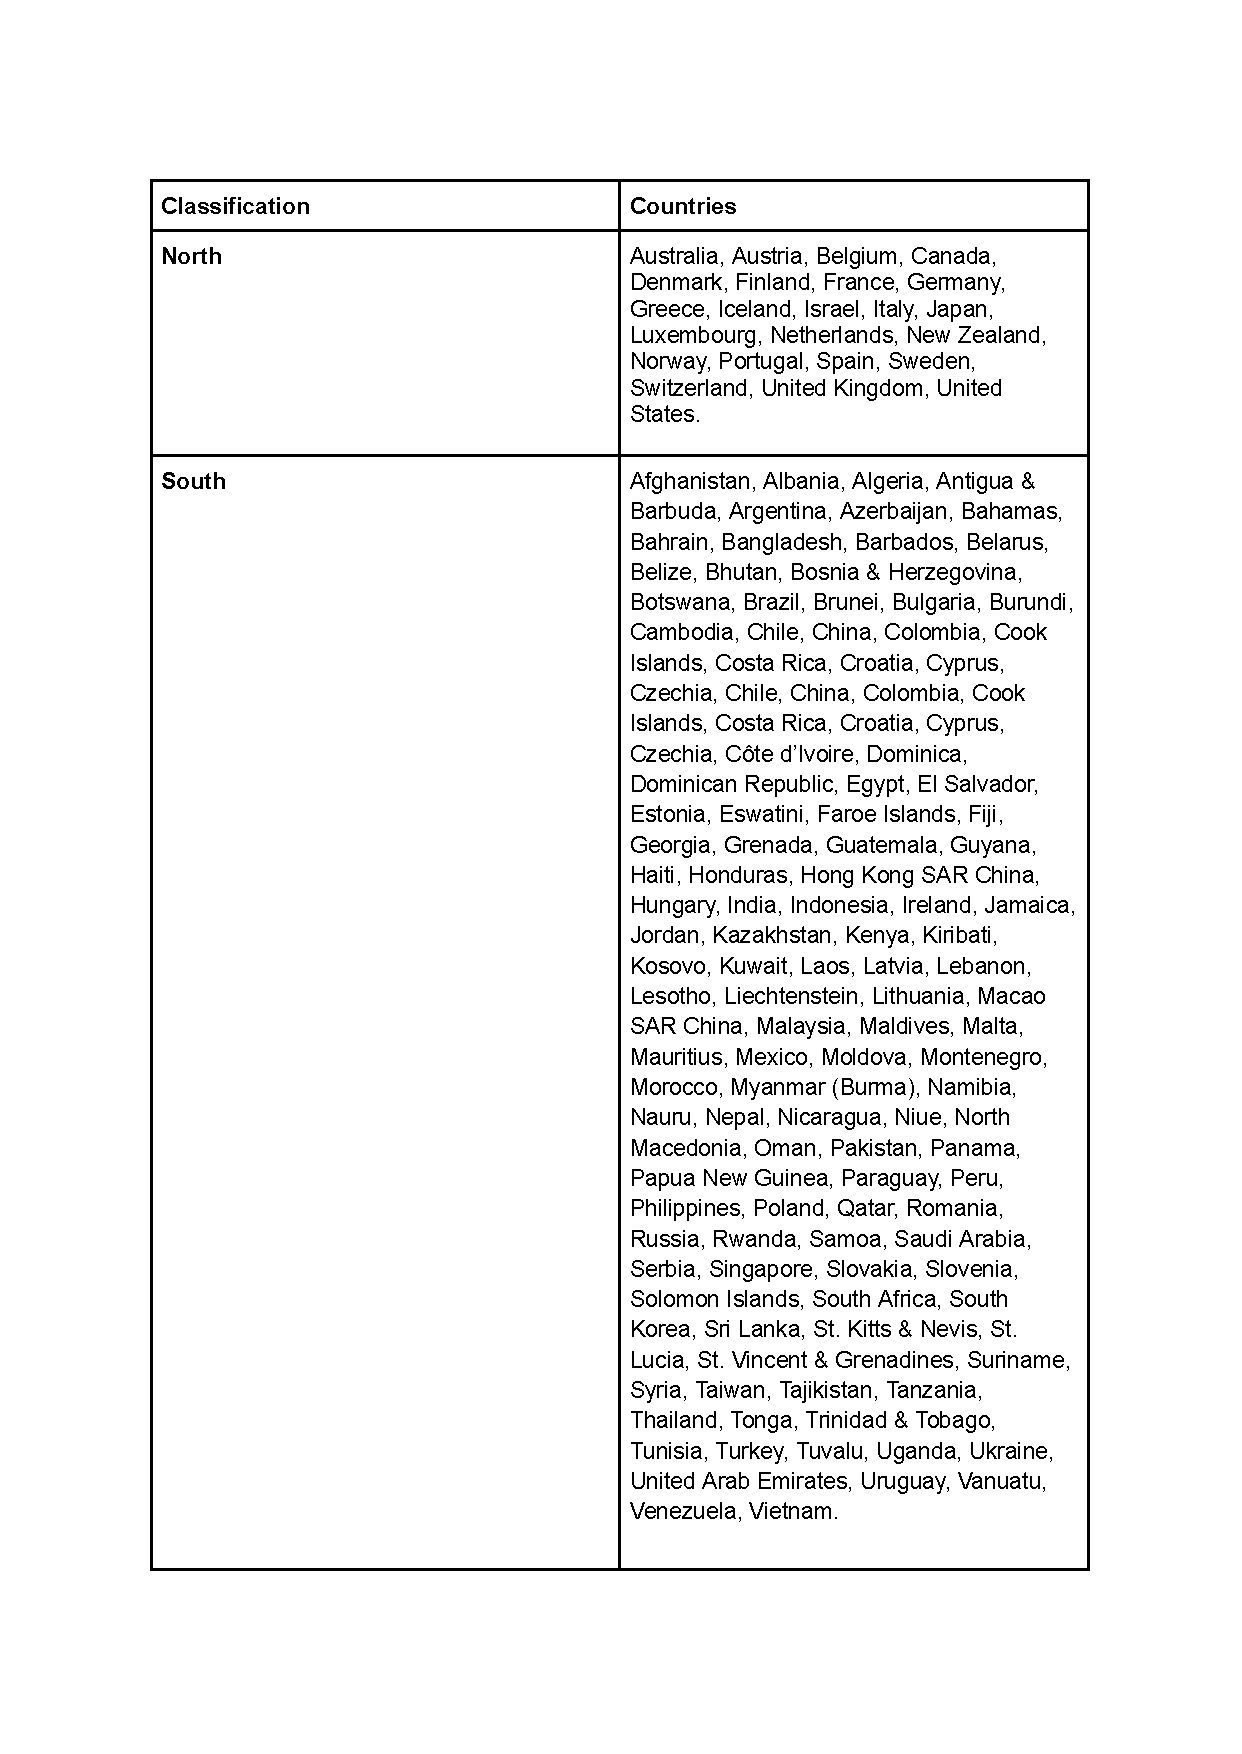
\includepdf[pages=-, fitpaper=true]{tables/countries.pdf}

%
\subsection{Appendix II {-} Sample TAs}%
\label{subsec:AppendixII{-}SampleTAs}%
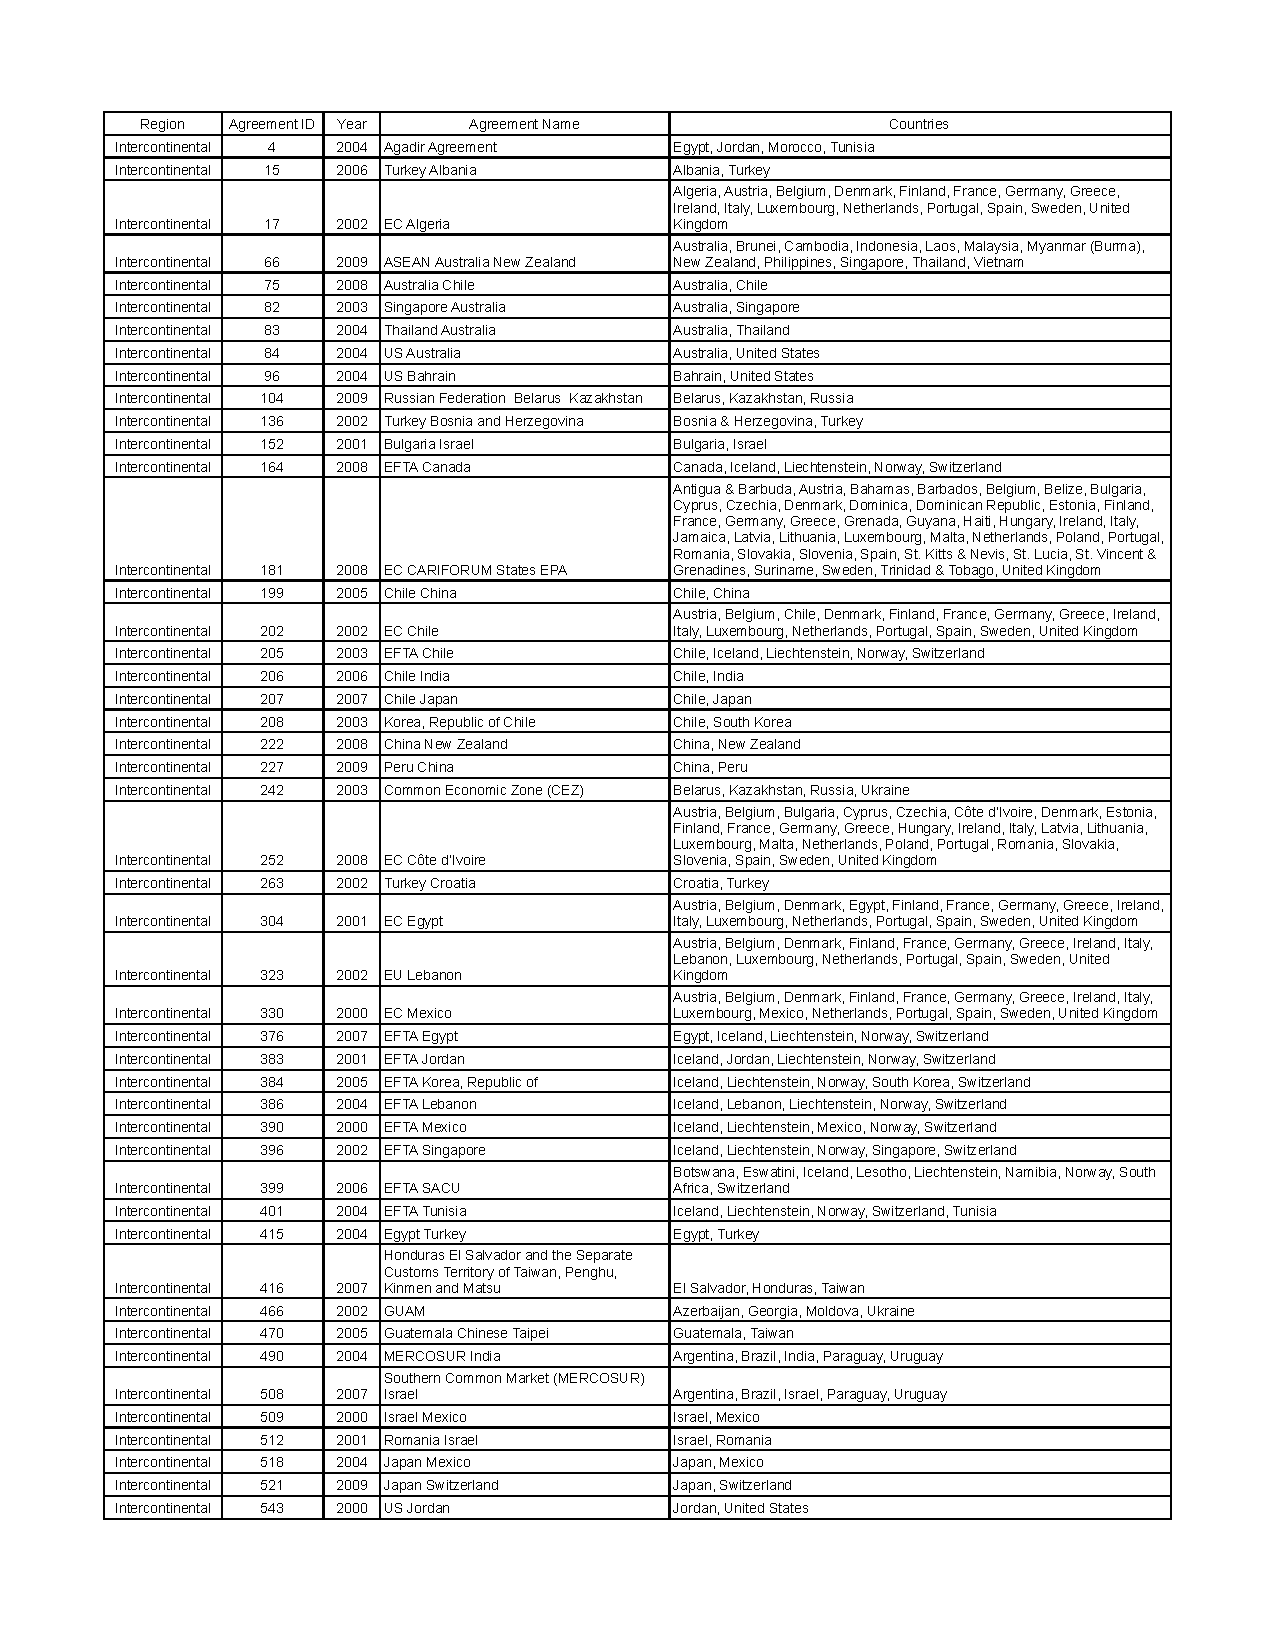
\includepdf[pages=-, fitpaper=true]{tables/pta_list.pdf}

%
\subsection{Appendix III {-} Regression Tables by Region for TA Heterogeneity Model}%
\label{subsec:AppendixIII{-}RegressionTablesbyRegionforTAHeterogeneityModel}%
\FloatBarrier%
\begin{table}[htbp]
    \centering
    \caption{PTA + PTA Lag Coefficients for Africa Region}
    \label{tab:pta_africa}
    \begin{adjustbox}{max width=\textwidth}
    \begin{tabular}{lcc}
    \hline
    \textbf{Statistically Insignificant} &  &  \\
    \hline
    PTA ID & Estimate & SE \\
    \hline
    670 & 0.326 & (0.410) \\
    787 & 0.304 & (0.233) \\
    \hline
    \multicolumn{3}{l}{\footnotesize{Notes: Robust standard errors clustered at the country-pair level in parentheses.}} \\
    \multicolumn{3}{l}{\footnotesize{Significance levels are indicated as follows: $^{\ast}$p$<$0.1; $^{\ast\ast}$p$<$0.05; $^{\ast\ast\ast}$p$<$0.01.}} \\
    \end{tabular}
    \end{adjustbox}
\end{table}
%
\FloatBarrier%
\begin{table}[htbp]
    \centering
    \caption{PTA + PTA Lag Coefficients for Americas Region}
    \label{tab:pta_americas}
    \begin{adjustbox}{max width=\textwidth}
    \begin{tabular}{lcc}
    \hline
    \textbf{Positive and Statistically Significant} &  &  \\
    \hline
    PTA ID & Estimate & SE \\
    \hline
    213 & 1.342$^{\ast\ast\ast}$ & (0.434) \\
    218 & 0.879$^{\ast\ast\ast}$ & (0.173) \\
    716 & 0.732$^{\ast\ast}$ & (0.358) \\
    239 & 0.571$^{\ast\ast\ast}$ & (0.173) \\
    201 & 0.545$^{\ast\ast}$ & (0.265) \\
    612 & 0.515$^{\ast\ast}$ & (0.251) \\
    616 & 0.488$^{\ast\ast\ast}$ & (0.044) \\
    168 & 0.410$^{\ast\ast\ast}$ & (0.113) \\
    163 & 0.342$^{\ast\ast\ast}$ & (0.096) \\
    141 & 0.265$^{\ast\ast\ast}$ & (0.024) \\
    \hline
    \textbf{Statistically Insignificant} &  &  \\
    \hline
    PTA ID & Estimate & SE \\
    \hline
    185 & 0.291 & (0.376) \\
    645 & 0.117 & (0.141) \\
    \hline
    \textbf{Negative and Statistically Significant} &  &  \\
    \hline
    PTA ID & Estimate & SE \\
    \hline
    188 & -0.774$^{\ast\ast\ast}$ & (0.144) \\
    \hline
    \multicolumn{3}{l}{\footnotesize{Notes: Robust standard errors clustered at the country-pair level in parentheses.}} \\
    \multicolumn{3}{l}{\footnotesize{Significance levels are indicated as follows: $^{\ast}$p$<$0.1; $^{\ast\ast}$p$<$0.05; $^{\ast\ast\ast}$p$<$0.01.}} \\
    \end{tabular}
    \end{adjustbox}
\end{table}
%
\FloatBarrier%
\begin{table}[htbp]
    \centering
    \caption{PTA + PTA Lag Coefficients for Asia Region}
    \label{tab:pta_asia}
    \begin{adjustbox}{max width=\textwidth}
    \begin{tabular}{lcc}
    \hline
    \textbf{Positive and Statistically Significant} &  &  \\
    \hline
    PTA ID & Estimate & SE \\
    \hline
    683 & 1.080$^{\ast\ast\ast}$ & (0.237) \\
    70  & 0.472$^{\ast\ast\ast}$ & (0.150) \\
    100 & 0.376$^{\ast\ast\ast}$ & (0.105) \\
    67  & 0.342$^{\ast\ast\ast}$ & (0.125) \\
    675 & 1.360$^{\ast\ast}$ & (0.655) \\
    475 & 0.636$^{\ast\ast}$ & (0.298) \\
    598 & 0.166$^{\ast\ast}$ & (0.083) \\
    474 & 0.419$^{\ast}$ & (0.243) \\
    \hline
    \textbf{Statistically Insignificant} &  &  \\
    \hline
    PTA ID & Estimate & SE \\
    \hline
    72  & 0.254 & (0.178) \\
    116 & 0.256 & (0.703) \\
    492 & 0.041 & (0.180) \\
    640 & 0.183 & (0.217) \\
    223 & -0.014 & (0.203) \\
    71  & -0.138 & (0.091) \\
    456 & -0.209 & (0.165) \\
    534 & -0.165 & (0.370) \\
    667 & -0.049 & (0.241) \\
    \hline
    \textbf{Negative and Statistically Significant} &  &  \\
    \hline
    PTA ID & Estimate & SE \\
    \hline
    221 & -2.955$^{\ast\ast\ast}$ & (0.727) \\
    220 & -1.215$^{\ast\ast\ast}$ & (0.093) \\
    599 & -0.967$^{\ast\ast\ast}$ & (0.191) \\
    1   & -0.732$^{\ast\ast}$ & (0.359) \\
    \hline
    Exporter-Year FE & Yes \\
    Importer-Year FE & Yes \\
    Country-Pair FE & Yes \\
    R-Squared & 0.999 \\
    Observations & 25308 \\
    \hline
    \multicolumn{3}{l}{\footnotesize{Notes: Robust standard errors clustered at the country-pair level in parentheses.}} \\
    \multicolumn{3}{l}{\footnotesize{Significance levels are indicated as follows: $^{\ast}$p$<$0.1; $^{\ast\ast}$p$<$0.05; $^{\ast\ast\ast}$p$<$0.01.}} \\
    \end{tabular}
    \end{adjustbox}
\end{table}
%
\FloatBarrier%
\begin{table}[htbp]
    \centering
    \caption{PTA + PTA Lag Coefficients for Europe Region}
    \label{tab:pta_europe}
    \begin{adjustbox}{max width=\textwidth}
    \begin{tabular}{lcc}
    \hline
    \textbf{Positive and Statistically Significant} &  &  \\
    \hline
    PTA ID & Estimate & SE \\
    \hline
    5   & 3.812$^{\ast\ast\ast}$ & (0.278) \\
    128 & 2.712$^{\ast\ast\ast}$ & (0.211) \\
    13  & 2.256$^{\ast\ast\ast}$ & (0.262) \\
    132 & 2.241$^{\ast\ast\ast}$ & (0.252) \\
    192 & 1.107$^{\ast\ast\ast}$ & (0.163) \\
    7   & 1.153$^{\ast\ast\ast}$ & (0.272) \\
    328 & 0.671$^{\ast\ast\ast}$ & (0.175) \\
    8   & 0.667$^{\ast\ast\ast}$ & (0.161) \\
    621 & 0.618$^{\ast\ast\ast}$ & (0.186) \\
    135 & 0.615$^{\ast\ast\ast}$ & (0.217) \\
    254 & 0.565$^{\ast\ast\ast}$ & (0.084) \\
    394 & 0.745$^{\ast\ast\ast}$ & (0.202) \\
    335 & 0.472$^{\ast\ast\ast}$ & (0.025) \\
    129 & 0.553$^{\ast\ast\ast}$ & (0.206) \\
    9   & 0.580$^{\ast\ast}$ & (0.285) \\
    11  & 0.656$^{\ast\ast}$ & (0.307) \\
    131 & 0.615$^{\ast\ast}$ & (0.281) \\
    594 & 0.474$^{\ast}$ & (0.251) \\
    \hline
    \textbf{Statistically Insignificant} &  &  \\
    \hline
    PTA ID & Estimate & SE \\
    \hline
    6   & 0.355 & (0.358) \\
    150 & 0.247 & (0.687) \\
    153 & 0.614 & (0.633) \\
    154 & 0.592 & (0.409) \\
    255 & 0.167 & (0.237) \\
    389 & 0.412 & (0.323) \\
    331 & 0.142 & (0.201) \\
    12  & -0.246 & (1.208) \\
    156 & -0.441 & (0.445) \\
    \hline
    \textbf{Negative and Statistically Significant} &  &  \\
    \hline
    PTA ID & Estimate & SE \\
    \hline
    133 & -0.772$^{\ast\ast\ast}$ & (0.248) \\
    \hline
    Exporter-Year FE & Yes \\
    Importer-Year FE & Yes \\
    Country-Pair FE & Yes \\
    R-Squared & 0.997 \\
    Observations & 28168 \\
    \hline
    \multicolumn{3}{l}{\footnotesize{Notes: Robust standard errors clustered at the country-pair level in parentheses.}} \\
    \multicolumn{3}{l}{\footnotesize{Significance levels are indicated as follows: $^{\ast}$p$<$0.1; $^{\ast\ast}$p$<$0.05; $^{\ast\ast\ast}$p$<$0.01.}} \\
    \end{tabular}
    \end{adjustbox} 
\end{table}
%
\FloatBarrier%
\begin{center}
\small
\begin{longtable}{lcc}
    \caption{PTA+PTALag Coefficients for Intercontinental} \label{tab:pta_intercontinental} \\
    
    \hline
    \textbf{Positive and Statistically Significant} &  &  \\
    \hline
    PTA ID & Estimate & SE \\
    \hline
    \endfirsthead
    
    \multicolumn{3}{c}{{\bfseries \tablename\ \thetable{} -- continued from previous page}} \\
    \hline
    PTA ID & Estimate & SE \\
    \hline
    \endhead
    
    \hline \multicolumn{3}{r}{{Continued on next page}} \\ \hline
    \endfoot
    
    \hline
    \endlastfoot
    
    627 & 2.372$^{\ast\ast\ast}$ & (0.345) \\
    415 & 1.853$^{\ast\ast\ast}$ & (0.201) \\
    206 & 1.539$^{\ast\ast\ast}$ & (0.180) \\
    75  & 1.366$^{\ast\ast\ast}$ & (0.493) \\
    263 & 1.426$^{\ast\ast\ast}$ & (0.115) \\
    4   & 1.254$^{\ast\ast\ast}$ & (0.268) \\
    626 & 1.099$^{\ast\ast\ast}$ & (0.121) \\
    657 & 0.705$^{\ast\ast\ast}$ & (0.082) \\
    637 & 0.667$^{\ast\ast\ast}$ & (0.102) \\
    202 & 0.658$^{\ast\ast\ast}$ & (0.123) \\
    208 & 0.763$^{\ast\ast\ast}$ & (0.129) \\
    136 & 0.744$^{\ast\ast\ast}$ & (0.185) \\
    490 & 0.843$^{\ast\ast\ast}$ & (0.181) \\
    17  & 0.811$^{\ast\ast\ast}$ & (0.242) \\
    466 & 0.710$^{\ast\ast\ast}$ & (0.147) \\
    304 & 0.770$^{\ast\ast\ast}$ & (0.120) \\
    628 & 0.484$^{\ast\ast\ast}$ & (0.142) \\
    207 & 0.516$^{\ast\ast\ast}$ & (0.114) \\
    518 & 0.627$^{\ast\ast\ast}$ & (0.135) \\
    330 & 0.314$^{\ast\ast\ast}$ & (0.086) \\
    164 & 0.288$^{\ast\ast\ast}$ & (0.073) \\
    96 & 0.271$^{\ast\ast\ast}$ & (0.055) \\
    181 & 0.392$^{\ast\ast}$ & (0.178) \\
    624 & 0.388$^{\ast\ast}$ & (0.163) \\
    521 & 0.101$^{\ast\ast}$ & (0.045) \\
    384  & 0.645$^{\ast}$ & (0.355) \\
    15  & 0.313$^{\ast}$ & (0.179) \\
    227 & 0.348$^{\ast}$ & (0.186) \\
    \hline
    \textbf{Statistically Insignificant} &  &  \\
    \hline
    PTA ID & Estimate & SE \\
    \hline
    641 & 2.028 & (1.255) \\
    543 & 1.090 & (0.707) \\
    509 & 0.210 & (0.216) \\
    252 & 0.192 & (0.357) \\
    508 & 0.140 & (0.122) \\
    376 & 0.172 & (0.228) \\
    416 & 0.424 & (0.295) \\
    401 & 0.407 & (0.288) \\
    152 & 0.110 & (0.266) \\
    242 & 0.050 & (0.294) \\
    390 & 0.0471 & (0.181) \\
    396 & 0.019 & (0.379) \\
    205 & 0.0012 & (0.178) \\
    602 & -0.076 & (0.918) \\
    383 & -0.202 & (0.152) \\
    386 & -0.092 & (0.168) \\
    84  & -0.059 & (0.120) \\
    979  & -0.126 & (0.294) \\
    644  & -0.189 & (0.122) \\
    658  & -0.303 & (0.349) \\
    \hline
    \textbf{Negative and Statistically Significant} &  &  \\
    \hline
    PTA ID & Estimate & SE \\
    \hline
    399 & -0.473$^{\ast\ast\ast}$ & (0.127) \\
    104 & -0.338$^{\ast\ast\ast}$ & (0.112) \\
    677 & -1.366$^{\ast\ast\ast}$ & (0.385) \\
    679 & -1.429$^{\ast\ast\ast}$ & (0.430) \\
    323 & -0.338$^{\ast\ast}$ & (0.138) \\
    512 & -0.458$^{\ast}$ & (0.266) \\
    \hline
    Exporter-Year FE & Yes \\
    Importer-Year FE & Yes \\
    Country-Pair FE & Yes \\
    R-Squared & 0.998 \\
    Observations & 73930 \\
    \hline
    \multicolumn{3}{l}{\footnotesize{Notes: Robust standard errors clustered at the country-pair level in parentheses.}} \\
    \multicolumn{3}{l}{\footnotesize{Significance levels are indicated as follows: $^{\ast}$p$<$0.1; $^{\ast\ast}$p$<$0.05; $^{\ast\ast\ast}$p$<$0.01.}} \\
\end{longtable}
\end{center}


% \begin{table}[htbp]
%     \centering
%     \caption{PTA + PTA Lag Coefficients for Intercontinental Region}
%     \label{tab:pta_intercontinental}
%     \begin{minipage}[t]{0.48\textwidth} % Adjust the width as needed
%         \centering
%         \begin{adjustbox}{max width=\textwidth}
%         \begin{tabular}{lcc}
%         \hline
%         \textbf{Positive and Statistically Significant} &  &  \\
%         \hline
%         PTA ID & Estimate & SE \\
%         \hline
%         627 & 2.372$^{\ast\ast\ast}$ & (0.345) \\
%         415 & 1.853$^{\ast\ast\ast}$ & (0.201) \\
%         206 & 1.539$^{\ast\ast\ast}$ & (0.180) \\
%         75  & 1.366$^{\ast\ast\ast}$ & (0.493) \\
%         263 & 1.426$^{\ast\ast\ast}$ & (0.115) \\
%         4   & 1.254$^{\ast\ast\ast}$ & (0.268) \\
%         626 & 1.099$^{\ast\ast\ast}$ & (0.121) \\
%         657 & 0.705$^{\ast\ast\ast}$ & (0.082) \\
%         637 & 0.667$^{\ast\ast\ast}$ & (0.102) \\
%         202 & 0.658$^{\ast\ast\ast}$ & (0.123) \\
%         208 & 0.763$^{\ast\ast\ast}$ & (0.129) \\
%         136 & 0.744$^{\ast\ast\ast}$ & (0.185) \\
%         490 & 0.843$^{\ast\ast\ast}$ & (0.181) \\
%         17  & 0.811$^{\ast\ast\ast}$ & (0.242) \\
%         466 & 0.710$^{\ast\ast\ast}$ & (0.147) \\
%         304 & 0.770$^{\ast\ast\ast}$ & (0.120) \\
%         628 & 0.484$^{\ast\ast\ast}$ & (0.142) \\
%         207 & 0.516$^{\ast\ast\ast}$ & (0.114) \\
%         518 & 0.627$^{\ast\ast\ast}$ & (0.135) \\
%         330 & 0.314$^{\ast\ast\ast}$ & (0.086) \\
%         164 & 0.288$^{\ast\ast\ast}$ & (0.073) \\
%         96 & 0.271$^{\ast\ast\ast}$ & (0.055) \\
%         181 & 0.392$^{\ast\ast}$ & (0.178) \\
%         624 & 0.388$^{\ast\ast}$ & (0.163) \\
%         521 & 0.101$^{\ast\ast}$ & (0.045) \\
%         384  & 0.645$^{\ast}$ & (0.355) \\
%         15  & 0.313$^{\ast}$ & (0.179) \\
%         227 & 0.348$^{\ast}$ & (0.186) \\
%         \hline
%         \end{tabular}
%         \end{adjustbox}
%     \end{minipage}%
%     \hfill
%     \begin{minipage}[t]{0.48\textwidth} % Adjust the width as needed
%         \centering
%         \begin{adjustbox}{max width=\textwidth}
%         \begin{tabular}{lcc}
%         \hline
%         \textbf{Statistically Insignificant} &  &  \\
%         \hline
%         PTA ID & Estimate & SE \\
%         \hline
%         641 & 2.028 & (1.255) \\
%         543 & 1.090 & (0.707) \\
%         509 & 0.210 & (0.216) \\
%         252 & 0.192 & (0.357) \\
%         508 & 0.140 & (0.122) \\
%         376 & 0.172 & (0.228) \\
%         416 & 0.424 & (0.295) \\
%         401 & 0.407 & (0.288) \\
%         152 & 0.110 & (0.266) \\
%         242 & 0.050 & (0.294) \\
%         390 & 0.0471 & (0.181) \\
%         396 & 0.019 & (0.379) \\
%         205 & 0.0012 & (0.178) \\
%         602 & -0.076 & (0.918) \\
%         383 & -0.202 & (0.152) \\
%         386 & -0.092 & (0.168) \\
%         84  & -0.059 & (0.120) \\
%         979  & -0.126 & (0.294) \\
%         644  & -0.189 & (0.122) \\
%         658  & -0.303 & (0.349) \\
%         \hline
%         \textbf{Negative and Statistically Significant} &  &  \\
%         \hline
%         PTA ID & Estimate & SE \\
%         \hline
%         399 & -0.473$^{\ast\ast\ast}$ & (0.127) \\
%         104 & -0.338$^{\ast\ast\ast}$ & (0.112) \\
%         677 & -1.366$^{\ast\ast\ast}$ & (0.385) \\
%         679 & -1.429$^{\ast\ast\ast}$ & (0.430) \\
%         323 & -0.338$^{\ast\ast}$ & (0.138) \\
%         512 & -0.458$^{\ast}$ & (0.266) \\
%         \hline
%         \end{tabular}
%         \end{adjustbox}
%     \end{minipage}
%     \vspace{0.5cm} % Optional: Add space between the tables and notes
%     \begin{adjustbox}{max width=\textwidth}
%     \begin{tabular}{l}
%     \hline
%     Exporter-Year FE & Yes \\
%     Importer-Year FE & Yes \\
%     Country-Pair FE & Yes \\
%     R-Squared & 0.998 \\
%     Observations & 73930 \\
%     \hline
%     \multicolumn{3}{l}{\footnotesize{Notes: Robust standard errors clustered at the country-pair level in parentheses.}} \\
%     \multicolumn{3}{l}{\footnotesize{Significance levels are indicated as follows: $^{\ast}$p$<$0.1; $^{\ast\ast}$p$<$0.05; $^{\ast\ast\ast}$p$<$0.01.}} \\
%     \end{tabular}
%     \end{adjustbox}
% \end{table}%
\FloatBarrier

%
\subsection{Appendix IV {-} Regression Tables by Region for TA Heterogeneity Extended Model}%
\label{subsec:AppendixIV{-}RegressionTablesbyRegionforTAHeterogeneityExtendedModel}%
\FloatBarrier%
\begin{table}[htbp]
    \centering
    \caption{Africa PTA + PTA Lag Coefficients by Type}
    \label{tab:africa_pta}
    \begin{adjustbox}{max width=\textwidth}
    \begin{tabular}{lccc}
    \hline
    \textbf{PTA ID} & \textbf{NS PTA + Lag} & \textbf{SS PTA + Lag} & \textbf{NN PTA + Lag} \\
    \hline
    \textbf{NS and SS (or only NS)} &  &  &  \\
    \hline
    \multicolumn{4}{c}{No agreements in this category} \\
    \hline
    \textbf{Only SS} &  &  &  \\
    \hline
    670 &  & 0.326 &  \\
     &  & (0.410) &  \\
    787 &  & 0.304 &  \\
     &  & (0.233) &  \\
    \hline
    \textbf{Agreements with NN and NS} &  &  &  \\
    \hline
    \multicolumn{4}{c}{No agreements in this category} \\
    \hline
    Exporter-Year FE & Yes \\
    Importer-Year FE & Yes \\
    Country-Pair FE & Yes \\
    R-Squared & 0.997 \\
    Observations & 5838 \\
    \hline
    \multicolumn{4}{l}{\footnotesize{Notes: Robust standard errors clustered at the country-pair level in parentheses.}} \\
    \multicolumn{4}{l}{\footnotesize{Significance levels are indicated as follows: $^{\ast}$p$<$0.1; $^{\ast\ast}$p$<$0.05; $^{\ast\ast\ast}$p$<$0.01.}} \\
    \end{tabular}
    \end{adjustbox}
\end{table}
%
\FloatBarrier%
\begin{table}[htbp]
    \centering
    \caption{Americas PTA + PTA Lag Coefficients by Type}
    \label{tab:americas_pta}
    \begin{adjustbox}{max width=\textwidth}
    \begin{tabular}{lccc}
    \hline
    \textbf{PTA ID} & \textbf{NS PTA+Lag} & \textbf{SS PTA+Lag} & \textbf{NN PTA+Lag} \\
    \hline
    \textbf{Agreements with NS and SS (or only NS)} &  &  &  \\
    \hline
    188 & -0.811$^{\ast\ast\ast}$ & 0.685$^{\ast\ast}$ &  \\
    & (0.140) & (0.317) & \\
    163 & 0.346$^{\ast\ast\ast}$ &  &  \\
    & (0.098) &  &  \\
    168 & 0.410$^{\ast\ast\ast}$ &  &  \\
    & (0.113) &  &  \\
    218 & 0.879$^{\ast\ast\ast}$ &  &  \\
    & (0.172) &  &  \\
    645 & 0.117 &  &  \\
    & (0.141) &  &  \\
    \hline
    \textbf{Agreements with only SS} &  &  &  \\
    \hline
    141 &  & 0.265$^{\ast\ast\ast}$ &  \\
    &  & (0.024) &  \\
    213 &  & 1.342$^{\ast\ast\ast}$ &  \\
    &  & (0.435) &  \\
    239 &  & 0.572$^{\ast\ast\ast}$ &  \\
    &  & (0.173) &  \\
    616 &  & 0.488$^{\ast\ast\ast}$ &  \\
    &  & (0.044) &  \\
    201 &  & 0.545$^{\ast\ast}$ &  \\
    &  & (0.265) &  \\
    716 &  & 0.732$^{\ast\ast}$ &  \\
    &  & (0.358) &  \\
    612 &  & 0.517$^{\ast\ast}$ &  \\
    &  & (0.251) &  \\
    185 &  & 0.295 &  \\
    &  & (0.375) &  \\
    \hline
    \textbf{Agreements with NN and NS} &  &  &  \\
    \hline
    \multicolumn{4}{c}{No agreements in this category} \\
    \hline
    Exporter-Year FE & Yes \\
    Importer-Year FE & Yes \\
    Country-Pair FE & Yes \\
    R-Squared & 0.999 \\
    Observations & 10997 \\
    \hline
    \multicolumn{4}{l}{\footnotesize{Notes: Robust standard errors clustered at the country-pair level in parentheses.}} \\
    \multicolumn{4}{l}{\footnotesize{Significance levels are indicated as follows: $^{\ast}$p$<$0.1; $^{\ast\ast}$p$<$0.05; $^{\ast\ast\ast}$p$<$0.01.}} \\
    \end{tabular}
    \end{adjustbox}
\end{table}
%
\FloatBarrier%
\begin{table}[htbp]
    \centering
    \caption{Asia PTA + PTA Lag Coefficients by Type}
    \label{tab:asia_pta}
    \begin{adjustbox}{max width=\textwidth}
    \begin{tabular}{lccc}
    \hline
    \textbf{PTA ID} & \textbf{NS PTA + Lag} & \textbf{SS PTA + Lag} & \textbf{NN PTA + Lag} \\
    \hline
    \textbf{Agreements with NS and SS (or only NS)} &  &  &  \\
    \hline
    598 & 0.166$^{\ast\ast}$ &  &  \\
    & (0.083) &  &  \\
    71 & -0.138 &  &  \\
    &  & (0.091) &  \\
    \hline
    \textbf{Agreements with only SS} &  &  &  \\
    \hline
    70 &  & 0.472$^{\ast\ast\ast}$ &  \\
    &  & (0.150) &  \\
    100 &  & 0.376$^{\ast\ast\ast}$ &  \\
    &  & (0.105) &  \\
    67 &  & 0.342$^{\ast\ast\ast}$ &  \\
    &  & (0.125) &  \\
    683 &  & 1.080$^{\ast\ast\ast}$ &  \\
    &  & (0.237) &  \\
    599 &  & -0.967$^{\ast\ast\ast}$ &  \\
    &  & (0.191) &  \\
    220 &  & -1.215$^{\ast\ast\ast}$ &  \\
    &  & (0.093) &  \\
    221 &  & -2.955$^{\ast\ast\ast}$ &  \\
    &  & (0.0.727) &  \\
    675 &  & 1.360$^{\ast\ast}$ &  \\
    &  & (0.655) &  \\
    475 &  & 0.636$^{\ast\ast}$ &  \\
    &  & (0.298) &  \\
    1 &  & -0.732$^{\ast\ast}$ &  \\
    &  & (0.359) &  \\
    474 &  & 0.419$^{\ast}$ &  \\
    &  & (0.243) &  \\
    116 &  & 0.256 &  \\
    &  & (0.703) &  \\
    72 & 0.254 &  &  \\
    &  & (0.178) &  \\
    492 & 0.041 &  &  \\
    &  & (0.180) &  \\
    640 & 0.183 &  &  \\
    &  & (0.217) &  \\
    667 & -0.049 &  &  \\
    &  & (0.241) &  \\
    534 & -0.165 &  &  \\
    &  & (0.370) &  \\
    223 & -0.014 &  &  \\
    &  & (0.203) &  \\
    456 & -0.209 &  &  \\
    &  & (0.165) &  \\
    \hline
    \textbf{Agreements with NN and NS} &  &  &  \\
    \hline
    \multicolumn{4}{c}{No agreements in this category} \\
    \hline
    Exporter-Year FE & Yes \\
    Importer-Year FE & Yes \\
    Country-Pair FE & Yes \\
    R-Squared & 0.999 \\
    Observations & 25308 \\
    \hline
    \multicolumn{4}{l}{\footnotesize{Notes: Robust standard errors clustered at the country-pair level in parentheses.}} \\
    \multicolumn{4}{l}{\footnotesize{Significance levels are indicated as follows: $^{\ast}$p$<$0.1; $^{\ast\ast}$p$<$0.05; $^{\ast\ast\ast}$p$<$0.01.}} \\
    \end{tabular}
    \end{adjustbox}
\end{table}
%
\FloatBarrier%
\begin{center}
\small
\begin{longtable}{lccc}
    \caption{Europe PTA + PTA Lag Coefficients by Type} \label{tab:europe_pta} \\

    \hline
    \textbf{Agreements with NS} &  &  &  \\
    \hline
    \textbf{PTA ID} & \textbf{NS PTA+Lag} & \textbf{SS PTA+Lag} & \textbf{NN PTA+Lag} \\
    \hline
    \endfirsthead
    
    \multicolumn{4}{c}{{\bfseries \tablename\ \thetable{} -- continued from previous page}} \\
    \hline
    \textbf{PTA ID} & \textbf{NS PTA+Lag} & \textbf{SS PTA+Lag} & \textbf{NN PTA+Lag} \\
    \hline
    \endhead
    
    \hline \multicolumn{4}{r}{{Continued on next page}} \\ \hline
    \endfoot
    
    \hline
    \endlastfoot
    
    8 & 0.663$^{\ast\ast\ast}$ & 0.783$^{\ast\ast\ast}$ &  \\
    & (0.165) & (0.248) &  \\
    254 & 0.568$^{\ast\ast\ast}$ & 0.323 &  \\
    & (0.086) & (0.430) &  \\
    328 & 0.738$^{\ast\ast\ast}$ & 0.354 &  \\
    & (0.179) & (0.291) &  \\
    331 & 0.241 & -0.032 &  \\
    & (0.216) & (0.338) &  \\
    394 & 0.747$^{\ast\ast\ast}$ &  &  \\
    & (0.200) &  &  \\
    9 & 0.581$^{\ast\ast}$ &  &  \\
    & (0.285) &  &  \\
    255 & 0.171 &  &  \\
    & (0.235) &  &  \\
    389 & 0.411 &  &  \\
    & (0.333) &  &  \\
    \hline
    \textbf{Agreements with only SS} &  &  &  \\
    \hline
    \textbf{PTA ID} & \textbf{NS PTA+Lag} & \textbf{SS PTA+Lag} & \textbf{NN PTA+Lag} \\
    \hline
    5   &  & 3.811$^{\ast\ast\ast}$ &  \\
    &  & (0.278) &  \\
    132 &  & 2.241$^{\ast\ast\ast}$ &  \\
    &  & (0.252) &  \\
    7   &  & 1.153$^{\ast\ast\ast}$ &  \\
    &  & (0.271) &  \\
    13  &  & 2.303$^{\ast\ast\ast}$ &  \\
    &  & (0.246) &  \\
    128 &  & 2.773$^{\ast\ast\ast}$ &  \\
    &  & (0.213) &  \\
    129 &  & 0.556$^{\ast\ast\ast}$ &  \\
    &  & (0.208) &  \\
    135 &  & 0.696$^{\ast\ast\ast}$ &  \\
    &  & (0.206) &  \\
    192 &  & 1.199$^{\ast\ast\ast}$ &  \\
    &  & (0.152) &  \\
    621 &  & 0.614$^{\ast\ast\ast}$ &  \\
    &  & (0.186) &  \\
    133 &  & -0.707$^{\ast\ast\ast}$ &  \\
    &  & (0.225) &  \\
    11  &  & 0.663$^{\ast\ast}$ &  \\
    &  & (0.298) &  \\
    131  &  & 0.599$^{\ast\ast}$ &  \\
    &  & (0.276) &  \\
    154  &  & 0.773$^{\ast\ast}$ &  \\
    &  & (0.354) &  \\
    594  &  & 0.455$^{\ast}$ &  \\
    &  & (0.249) &  \\
    150 &  & 0.444 &  \\
    &  & (0.679) &  \\
    153 &  & 0.817 &  \\
    &  & (0.596) &  \\
    6   &  & 0.411 &  \\
    &  & (0.352) &  \\
    156   &  & -0.372 &  \\
    &  & (0.428) &  \\
    12   &  & -0.250 &  \\
    &  & (1.207) &  \\
    \hline
    \textbf{Agreements with NN} &  &  &  \\
    \hline
    \textbf{PTA ID} & \textbf{NS PTA+Lag} & \textbf{SS PTA+Lag} & \textbf{NN PTA+Lag} \\
    \hline
    335 & 0.727$^{\ast\ast\ast}$ & 1.099$^{\ast\ast\ast}$ & 0.399$^{\ast\ast\ast}$ \\
    & (0.047) & (0.098) & (0.025) \\
    \hline
    Exporter-Year FE & Yes \\
    Importer-Year FE & Yes \\
    Country-Pair FE & Yes \\
    R-Squared & 0.997 \\
    Observations & 28168 \\
    \hline
    \multicolumn{4}{l}{\footnotesize{Notes: Robust standard errors clustered at the country-pair level in parentheses.}} \\
    \multicolumn{4}{l}{\footnotesize{Significance levels are indicated as follows: $^{\ast}$p$<$0.1; $^{\ast\ast}$p$<$0.05; $^{\ast\ast\ast}$p$<$0.01.}} \\
\end{longtable}
\end{center}


% \begin{table}[htbp]
%     \centering
%     \caption{Europe PTA + PTA Lag Coefficients by Type}
%     \label{tab:europe_pta}
%     \begin{adjustbox}{max width=\textwidth}
%     \begin{tabular}{lccc}
%     \hline
%     \textbf{PTA ID} & \textbf{NS PTA+Lag} & \textbf{SS PTA+Lag} & \textbf{NN PTA+Lag} \\
%     \hline
%     \textbf{Agreements with NS} &  &  &  \\
%     \hline
%     8   & 0.663$^{\ast\ast\ast}$ & 0.783$^{\ast\ast\ast}$ &  \\
%     & (0.165) & (0.248) &  \\
%     254 & 0.568$^{\ast\ast\ast}$ & 0.323 &  \\
%     & (0.086) & (0.430) &  \\
%     328 & 0.738$^{\ast\ast\ast}$ & 0.354 &  \\
%     & (0.179) & (0.291) &  \\
%     394 & 0.747$^{\ast\ast\ast}$ &  &  \\
%     &  & (0.200) &  \\
%     9   & 0.581$^{\ast\ast}$ &  &  \\
%     & (0.285) &  &  \\
%     331   & 0.241 & -0.032 &  \\
%     & (0.216) & (0.338) &  \\
%     255   & 0.171 &  &  \\
%     & (0.235) &  &  \\
%     389   & 0.411 &  &  \\
%     & (0.333) &  &  \\
%     \hline
%     \textbf{Agreements with only SS} &  &  &  \\
%     \hline
%     5   &  & 3.811$^{\ast\ast\ast}$ &  \\
%     &  & (0.278) &  \\
%     132 &  & 2.241$^{\ast\ast\ast}$ &  \\
%     &  & (0.252) &  \\
%     7   &  & 1.153$^{\ast\ast\ast}$ &  \\
%     &  & (0.271) &  \\
%     13  &  & 2.303$^{\ast\ast\ast}$ &  \\
%     &  & (0.246) &  \\
%     128 &  & 2.773$^{\ast\ast\ast}$ &  \\
%     &  & (0.213) &  \\
%     129 &  & 0.556$^{\ast\ast\ast}$ &  \\
%     &  & (0.208) &  \\
%     135 &  & 0.696$^{\ast\ast\ast}$ &  \\
%     &  & (0.206) &  \\
%     192 &  & 1.199$^{\ast\ast\ast}$ &  \\
%     &  & (0.152) &  \\
%     621 &  & 0.614$^{\ast\ast\ast}$ &  \\
%     &  & (0.186) &  \\
%     133 &  & -0.707$^{\ast\ast\ast}$ &  \\
%     &  & (0.225) &  \\
%     11  &  & 0.663$^{\ast\ast}$ &  \\
%     &  & (0.298) &  \\
%     131  &  & 0.599$^{\ast\ast}$ &  \\
%     &  & (0.276) &  \\
%     154  &  & 0.773$^{\ast\ast}$ &  \\
%     &  & (0.354) &  \\
%     594  &  & 0.455$^{\ast}$ &  \\
%     &  & (0.249) &  \\
%     150 &  & 0.444 &  \\
%     &  & (0.679) &  \\
%     153 &  & 0.817 &  \\
%     &  & (0.596) &  \\
%     6   &  & 0.411 &  \\
%     &  & (0.352) &  \\
%     156   &  & -0.372 &  \\
%     &  & (0.428) &  \\
%     12   &  & -0.250 &  \\
%     &  & (1.207) &  \\
%     \hline
%     \textbf{Agreements with NN} &  &  &  \\
%     \hline
%     335 & 0.727$^{\ast\ast\ast}$ & 1.099$^{\ast\ast\ast}$ & 0.399$^{\ast\ast\ast}$ \\
%     & (0.047) & (0.098) & (0.025) \\
%     \hline
%     Exporter-Year FE & Yes \\
%     Importer-Year FE & Yes \\
%     Country-Pair FE & Yes \\
%     R-Squared & 0.997 \\
%     Observations & 28168 \\
%     \hline
%     \multicolumn{4}{l}{\footnotesize{Notes: Robust standard errors clustered at the country-pair level in parentheses.}} \\
%     \multicolumn{4}{l}{\footnotesize{Significance levels are indicated as follows: $^{\ast}$p$<$0.1; $^{\ast\ast}$p$<$0.05; $^{\ast\ast\ast}$p$<$0.01.}} \\
%     \end{tabular}
%     \end{adjustbox}
% \end{table}
%
\FloatBarrier%
\begin{center}
\small
\begin{longtable}{lccc}
    \caption{Intercont PTA+Lag Coefficients by Type} \label{tab:intercontinental_pta} \\

    \hline
    \textbf{Agreements with NS} &  &  &  \\
    \hline
    \textbf{PTA ID} & \textbf{NS PTA+Lag} & \textbf{SS PTA+Lag} & \textbf{NN PTA+Lag} \\
    \hline
    \endfirsthead
    
    \multicolumn{4}{c}{{\bfseries \tablename\ \thetable{} -- continued from previous page}} \\
    \hline
    \textbf{PTA ID} & \textbf{NS PTA+Lag} & \textbf{SS PTA+Lag} & \textbf{NN PTA+Lag} \\
    \hline
    \endhead
    
    \hline \multicolumn{4}{r}{{Continued on next page}} \\ \hline
    \endfoot
    
    \hline
    \endlastfoot
    
    17  & 0.800$^{\ast\ast\ast}$ & 1.055$^{\ast\ast\ast}$ &  \\
    & (0.249) & (0.244) &  \\
    330 & 0.286$^{\ast\ast\ast}$ & 0.662$^{\ast\ast\ast}$ &  \\
    & (0.088) & (0.188) &  \\
    304 & 0.787$^{\ast\ast\ast}$ & 0.591$^{\ast\ast}$ &  \\
    & (0.123) & (0.245) &  \\
    202 & 0.660$^{\ast\ast\ast}$ & 0.612$^{\ast\ast}$ &  \\
    & (0.124) & (0.241) &  \\
    679 & 0.546$^{\ast}$ & -1.636$^{\ast\ast\ast}$ &  \\
    & (0.310) & (0.400) &  \\
    323 & -0.335$^{\ast\ast}$ & -0.360 &  \\
    & (0.146) & (0.247) &  \\
    181 & 0.242 & 1.288$^{\ast\ast\ast}$ &  \\
    & (0.179) & (0.309) &  \\
    252 & 0.165 & 0.580 &  \\
    & (0.363) & (0.387) &  \\
    979 & -0.130 & 0.061 &  \\
    & (0.298) & (0.855) &  \\
    75  & 1.366$^{\ast\ast\ast}$ &  &  \\
    & (0.492) &  &  \\
    96  & 0.271$^{\ast\ast\ast}$ &  &  \\
    & (0.055) &  &  \\
    207 & 0.516$^{\ast\ast\ast}$ &  &  \\
    & (0.113) &  &  \\
    518 & 0.627$^{\ast\ast\ast}$ &  &  \\
    & (0.135) &  &  \\
    628 & 0.484$^{\ast\ast\ast}$ &  &  \\
    & (0.142) &  &  \\
    637 & 0.667$^{\ast\ast\ast}$ &  &  \\
    & (0.102) &  &  \\
    399 & -0.473$^{\ast\ast\ast}$ &  &  \\
    & (0.127) &  &  \\
    384 & 0.645$^{\ast}$ &  &  \\
    & (0.355) &  &  \\
    512 & -0.458$^{\ast}$ &  &  \\
    & (0.266) &  &  \\
    543 & 1.090 &  &  \\
    & (0.707) &  &  \\
    376 & 0.171 &  &  \\
    & (0.228) &  &  \\
    152 & 0.110 &  &  \\
    & (0.266) &  &  \\
    205 & 0.002 &  &  \\
    & (0.178) &  &  \\
    390 & 0.047 &  &  \\
    & (0.181) &  &  \\
    396 & 0.018 &  &  \\
    & (0.379) &  &  \\
    401 & 0.407 &  &  \\
    & (0.288) &  &  \\
    508 & 0.140 &  &  \\
    & (0.122) &  &  \\
    509 & 0.210 &  &  \\
    & (0.216) &  &  \\
    658 & -0.303 &  &  \\
    & (0.349) &  &  \\
    383 & -0.202 &  &  \\
    & (0.152) &  &  \\
    386 & -0.092 &  &  \\
    & (0.168) &  &  \\
    \hline
    \textbf{Agreements with only SS} &  &  &  \\
    \hline
    \textbf{PTA ID} & \textbf{NS PTA+Lag} & \textbf{SS PTA+Lag} & \textbf{NN PTA+Lag} \\
    \hline
    627 &  & 2.372$^{\ast\ast\ast}$ &  \\
    &  & (0.345) &  \\
    415   &  & 1.854$^{\ast\ast\ast}$ &  \\
    &  & (0.201) &  \\
    4   &  & 1.255$^{\ast\ast\ast}$ &  \\
    &  & (0.268) &  \\
    626 &  & 1.099$^{\ast\ast\ast}$ &  \\
    &  & (0.121) &  \\
    104 &  & -0.338$^{\ast\ast\ast}$ &  \\
    &  & (0.112) &  \\
    136 &  & 0.744$^{\ast\ast\ast}$ &  \\
    &  & (0.185) &  \\
    208 &  & 0.763$^{\ast\ast\ast}$ &  \\
    &  & (0.129) &  \\
    657 &  & 0.705$^{\ast\ast\ast}$ &  \\
    &  & (0.082) &  \\
    206 &  & 1.540$^{\ast\ast\ast}$ &  \\
    &  & (0.180) &  \\
    263 &  & 1.426$^{\ast\ast\ast}$ &  \\
    &  & (0.115) &  \\
    466 &  & 0.710$^{\ast\ast\ast}$ &  \\
    &  & (0.147) &  \\
    490 &  & 0.843$^{\ast\ast\ast}$ &  \\
    &  & (0.181) &  \\
    677 &  & -1.366$^{\ast\ast\ast}$ &  \\
    &  & (0.385) &  \\
    624 &  & 0.384$^{\ast\ast}$ &  \\
    &  & (0.163) &  \\
    15  &  & 0.313$^{\ast}$ &  \\
    &  & (0.179) &  \\
    227  &  & 0.348$^{\ast}$ &  \\
    &  & (0.186) &  \\
    242  &  & 0.050 &  \\
    &  & (0.294) &  \\
    416  &  & 0.424 &  \\
    &  & (0.295) &  \\
    641  &  & 2.027 &  \\
    &  & (1.255) &  \\
    644  &  & -0.190 &  \\
    &  & (0.122) &  \\
    602  &  & -0.076 &  \\
    &  & (0.918) &  \\
    \hline
    \textbf{Agreements with NN} &  &  &  \\
    \hline
    \textbf{PTA ID} & \textbf{NS PTA+Lag} & \textbf{SS PTA+Lag} & \textbf{NN PTA+Lag} \\
    \hline
    164 &  &  & 0.288$^{\ast\ast\ast}$ \\
    &  &  & (0.073) \\
    521 &  &  & 0.102$^{\ast\ast}$ \\
    &  &  & (0.045) \\
    84  &  &  & -0.059 \\
    &  &  & (0.120) \\
    \hline
    Exporter-Year FE & Yes \\
    Importer-Year FE & Yes \\
    Country-Pair FE & Yes \\
    R-Squared & 0.998 \\
    Observations & 73930 \\
    \hline
    \multicolumn{4}{l}{\footnotesize{Notes: Robust standard errors clustered at the country-pair level in parentheses.}} \\
    \multicolumn{4}{l}{\footnotesize{Significance levels are indicated as follows: $^{\ast}$p$<$0.1; $^{\ast\ast}$p$<$0.05; $^{\ast\ast\ast}$p$<$0.01.}} \\
\end{longtable}
\end{center}

% \begin{table}[htbp]
%     \centering
%     \caption{Intercontinental PTA + PTA Lag Coefficients by Type}
%     \label{tab:intercontinental_pta}
%     \begin{adjustbox}{max width=\textwidth}
%     \begin{tabular}{lccc}
%     \hline
%     \textbf{PTA ID} & \textbf{NS PTA + Lag} & \textbf{SS PTA + Lag} & \textbf{NN PTA + Lag} \\
%     \hline
%     \textbf{Agreements with NS and SS (or only NS)} &  &  &  \\
%     \hline
%     75  & 1.366$^{\ast\ast\ast}$ &  &  \\
%     & (0.492) &  &  \\
%     96  & 0.271$^{\ast\ast\ast}$ &  &  \\
%     & (0.055) &  &  \\
%     207 & 0.516$^{\ast\ast\ast}$ &  &  \\
%     & (0.113) &  &  \\
%     518 & 0.627$^{\ast\ast\ast}$ &  &  \\
%     & (0.135) &  &  \\
%     628 & 0.484$^{\ast\ast\ast}$ &  &  \\
%     & (0.142) &  &  \\
%     637 & 0.667$^{\ast\ast\ast}$ &  &  \\
%     & (0.102) &  &  \\
%     399 & -0.473$^{\ast\ast\ast}$ &  &  \\
%     & (0.127) &  &  \\
%     384 & 0.645$^{\ast}$ &  &  \\
%     & (0.355) &  &  \\
%     512 & -0.458$^{\ast}$ &  &  \\
%     & (0.266) &  &  \\
%     17  & 0.800$^{\ast\ast\ast}$ & 1.055$^{\ast\ast\ast}$ &  \\
%     & (0.249) & (0.244) &  \\
%     330 & 0.286$^{\ast\ast\ast}$ & 0.662$^{\ast\ast\ast}$ &  \\
%     & (0.088) & (0.188) &  \\
%     304 & 0.787$^{\ast\ast\ast}$ & 0.591$^{\ast\ast}$ &  \\
%     & (0.123) & (0.245) &  \\
%     202 & 0.660$^{\ast\ast\ast}$ & 0.612$^{\ast\ast}$ &  \\
%     & (0.124) & (0.241) &  \\
%     679 & 0.546$^{\ast}$ & -1.636$^{\ast\ast\ast}$ &  \\
%     & (0.310) & (0.400) &  \\
%     323 & -0.335$^{\ast\ast}$ & -0.360 &  \\
%     & (0.146) & (0.247) &  \\
%     181 & 0.242 & 1.288$^{\ast\ast\ast}$ &  \\
%     & (0.179) & (0.309) &  \\
%     252 & 0.165 & 0.580 &  \\
%     & (0.363) & (0.387) &  \\
%     979 & -0.130 & 0.061 &  \\
%     & (0.298) & (0.855) &  \\
%     543 & 1.090 &  &  \\
%     & (0.707) &  &  \\
%     376 & 0.171 &  &  \\
%     & (0.228) &  &  \\
%     152 & 0.110 &  &  \\
%     & (0.266) &  &  \\
%     205 & 0.002 &  &  \\
%     & (0.178) &  &  \\
%     390 & 0.047 &  &  \\
%     & (0.181) &  &  \\
%     396 & 0.018 &  &  \\
%     & (0.379) &  &  \\
%     401 & 0.407 &  &  \\
%     & (0.288) &  &  \\
%     508 & 0.140 &  &  \\
%     & (0.122) &  &  \\
%     509 & 0.210 &  &  \\
%     & (0.216) &  &  \\
%     658 & -0.303 &  &  \\
%     & (0.349) &  &  \\
%     383 & -0.202 &  &  \\
%     & (0.152) &  &  \\
%     386 & -0.092 &  &  \\
%     & (0.168) &  &  \\
%     \hline
%     \textbf{Agreements with only SS} &  &  &  \\
%     \hline
%     627 &  & 2.372$^{\ast\ast\ast}$ &  \\
%     &  & (0.345) &  \\
%     415   &  & 1.854$^{\ast\ast\ast}$ &  \\
%     &  & (0.201) &  \\
%     4   &  & 1.255$^{\ast\ast\ast}$ &  \\
%     &  & (0.268) &  \\
%     626 &  & 1.099$^{\ast\ast\ast}$ &  \\
%     &  & (0.121) &  \\
%     104 &  & -0.338$^{\ast\ast\ast}$ &  \\
%     &  & (0.112) &  \\
%     136 &  & 0.744$^{\ast\ast\ast}$ &  \\
%     &  & (0.185) &  \\
%     208 &  & 0.763$^{\ast\ast\ast}$ &  \\
%     &  & (0.129) &  \\
%     657 &  & 0.705$^{\ast\ast\ast}$ &  \\
%     &  & (0.082) &  \\
%     206 &  & 1.540$^{\ast\ast\ast}$ &  \\
%     &  & (0.180) &  \\
%     263 &  & 1.426$^{\ast\ast\ast}$ &  \\
%     &  & (0.115) &  \\
%     466 &  & 0.710$^{\ast\ast\ast}$ &  \\
%     &  & (0.147) &  \\
%     490 &  & 0.843$^{\ast\ast\ast}$ &  \\
%     &  & (0.181) &  \\
%     677 &  & -1.366$^{\ast\ast\ast}$ &  \\
%     &  & (0.385) &  \\
%     624 &  & 0.384$^{\ast\ast}$ &  \\
%     &  & (0.163) &  \\
%     15  &  & 0.313$^{\ast}$ &  \\
%     &  & (0.179) & () \\
%     227  &  & 0.348$^{\ast}$ &  \\
%     &  & (0.186) &  \\
%     242  &  & 0.050 &  \\
%     &  & (0.294) &  \\
%     416  &  & 0.424 &  \\
%     &  & (0.295) &  \\
%     641  &  & 2.027 &  \\
%     &  & (1.255) &  \\
%     644  &  & -0.190 &  \\
%     &  & (0.122) &  \\
%     602  &  & -0.076 &  \\
%     &  & (0.918) &  \\
%     \hline
%     \textbf{Agreements with NN and NS} &  &  &  \\
%     \hline
%     164 &  &  & 0.288$^{\ast\ast\ast}$ \\
%     &  &  & (0.073) \\
%     521 &  &  & 0.102$^{\ast\ast}$ \\
%     &  &  & (0.045) \\
%     84  &  &  & -0.059 \\
%     &  &  & (0.120) \\
%     \hline
%     Exporter-Year FE & Yes \\
%     Importer-Year FE & Yes \\
%     Country-Pair FE & Yes \\
%     R-Squared & 0.998 \\
%     Observations & 73930 \\
%     \hline
%     \multicolumn{4}{l}{\footnotesize{Notes: Robust standard errors clustered at the country-pair level in parentheses.}} \\
%     \multicolumn{4}{l}{\footnotesize{Significance levels are indicated as follows: $^{\ast}$p$<$0.1; $^{\ast\ast}$p$<$0.05; $^{\ast\ast\ast}$p$<$0.01.}} \\
%     \end{tabular}
%     \end{adjustbox}
% \end{table}%
\FloatBarrier

%
%TC:endignore%
\end{document}